% This is "sig-alternate.tex" V2.1 April 2013
% This file should be compiled with V2.5 of "sig-alternate.cls" May 2012
%
% This example file demonstrates the use of the 'sig-alternate.cls'
% V2.5 LaTeX2e document class file. It is for those submitting
% articles to ACM Conference Proceedings WHO DO NOT WISH TO
% STRICTLY ADHERE TO THE SIGS (PUBS-BOARD-ENDORSED) STYLE.
% The 'sig-alternate.cls' file will produce a similar-looking,
% albeit, 'tighter' paper resulting in, invariably, fewer pages.
%
% ----------------------------------------------------------------------------------------------------------------
% This .tex file (and associated .cls V2.5) produces:
%       1) The Permission Statement
%       2) The Conference (location) Info information
%       3) The Copyright Line with ACM data
%       4) NO page numbers
%
% as against the acm_proc_article-sp.cls file which
% DOES NOT produce 1) thru' 3) above.
%
% Using 'sig-alternate.cls' you have control, however, from within
% the source .tex file, over both the CopyrightYear
% (defaulted to 200X) and the ACM Copyright Data
% (defaulted to X-XXXXX-XX-X/XX/XX).
% e.g.
% \CopyrightYear{2007} will cause 2007 to appear in the copyright line.
% \crdata{0-12345-67-8/90/12} will cause 0-12345-67-8/90/12 to appear in the copyright line.
%
% ---------------------------------------------------------------------------------------------------------------
% This .tex source is an example which *does* use
% the .bib file (from which the .bbl file % is produced).
% REMEMBER HOWEVER: After having produced the .bbl file,
% and prior to final submission, you *NEED* to 'insert'
% your .bbl file into your source .tex file so as to provide
% ONE 'self-contained' source file.
%
% ================= IF YOU HAVE QUESTIONS =======================
% Questions regarding the SIGS styles, SIGS policies and
% procedures, Conferences etc. should be sent to
% Adrienne Griscti (griscti@acm.org)
%
% Technical questions _only_ to
% Gerald Murray (murray@hq.acm.org)
% ===============================================================
%
% For tracking purposes - this is V2.0 - May 2012

\documentclass[sigconf]{acmart}

\usepackage{booktabs} % For formal tables
% DOI
%\acmDOI{10.475/123_4}

% ISBN
%\acmISBN{123-4567-24-567/08/06}

%Conference
%\acmConference[WOODSTOCK'97]{ACM Woodstock conference}{July 1997}{El
%  Paso, Texas USA} 
\acmYear{2018}
%\copyrightyear{2016}

\usepackage{url}
\usepackage{lipsum}% http://ctan.org/pkg/lipsum
\usepackage{graphicx}% http://ctan.org/pkg/graphicx
\usepackage{color,soul}
\usepackage{float}
\usepackage{amsmath}
\usepackage[disable]{todonotes}
\usepackage[outdir=./figures/]{epstopdf}
\usepackage{listings}
\PassOptionsToPackage{table}{colorx}
\usepackage{booktabs}
\usepackage{subcaption}
\usepackage{upquote}
\makeatletter
\def\@copyrightspace{\relax}
\makeatother
\DeclareMathOperator*{\argmin}{arg\,min}
\begin{document}
%\lstset{numbers=left, numberstyle=\small, numbersep=8pt, frame = single, language=Pascal, framexleftmargin=15pt}

\title{Continuous Training of Deployed Machine Learning Models}

%
% You need the command \numberofauthors to handle the 'placement
% and alignment' of the authors beneath the title.
%
% For aesthetic reasons, we recommend 'three authors at a time'
% i.e. three 'name/affiliation blocks' be placed beneath the title.
%
% NOTE: You are NOT restricted in how many 'rows' of
% "name/affiliations" may appear. We just ask that you restrict
% the number of 'columns' to three.
%
% Because of the available 'opening page real-estate'
% we ask you to refrain from putting more than six authors
% (two rows with three columns) beneath the article title.
% More than six makes the first-page appear very cluttered indeed.
%
% Use the \alignauthor commands to handle the names
% and affiliations for an 'aesthetic maximum' of six authors.
% Add names, affiliations, addresses for
% the seventh etc. author(s) as the argument for the
% \additionalauthors command.
% These 'additional authors' will be output/set for you
% without further effort on your part as the last section in
% the body of your article BEFORE References or any 


%
%
%\author{Behrouz Derakhshan}
%\affiliation{%
%  \institution{DFKI, Germany}
%}
%\email{behrouz.derakhshan@dfki.de}
%
%\author{Tilmann Rabl}
%\affiliation{%
%  \institution{DFKI, Germany}
%}
%\additionalaffiliation{
%\institution{TU Berlin, Germany, rabl@tu-berlin.de}
%}
%\email{tilmann.rabl@dfki.de}
%
%\author{Volker Markl}
%\affiliation{%
%  \institution{DFKI, Germany}
%}
%\additionalaffiliation{%
%  \institution{TU Berlin, Germany, volker.markl@tu-berlin.de}
%}
%\email{volker.markl@dfki.de}
%
%
%\author{Author 1}
%\affiliation{%
%  \institution{DFKI, Germany}
%}
%%\email{behrouz.derakhshan@dfki.de}
%\author{Author 2}
%\affiliation{%
%  \institution{DFKI, Germany}
%}
%\additionalaffiliation{%
%  \institution{TU Berlin, Germany}
%}
%%\email{tilmann.rabl@dfki.de}
%\author{Author 3}
%\affiliation{%
%  \institution{DFKI, Germany}
%}
%\additionalaffiliation{%
%  \institution{TU Berlin, Germany}
%}
%\email{volker.markl@dfki.de}

\begin{abstract}
Today machine learning is entering many business and scientific applications.
The life cycle of machine learning applications consist of data preprocessing for transforming the raw data into features, training a model using the features, and deploying the model for answering prediction queries.
In order to guarantee accurate predictions, one has to continuously monitor and update the deployed models and pipelines. 
Current deployment platforms update the models using online learning methods.
When online learning alone is not adequate to guarantee the prediction accuracy, some deployment systems provide a mechanism for automatic or manual retraining the model.
While the online training is fast, the retraining of the model is time-consuming and adds extra overhead and complexity to the process of deployment.

We propose a novel approach for continuously updating the deployed model using a combination of the incoming real-time data and the historical data.
We utilize fast sampling techniques to include the historical data in the training process, thus eliminating the need for complete retraining of deployed model.
Moreover, we offer several optimizations such as online statistics computation and materialization of preprocessed features to minimize the total training and data preprocessing time.
\todo[inline]{make it more explicit, two dataset two models, we improve error and reduce time}
In our experiments, we show that our continuous training approach updates the model more frequently while using fewer resources.
As a result, the continuous deployment improves the error rate of the deployed model up to 0.3\%  and reduces the total training cost up to 13 times over the state-of-the-art deployment approaches.
\end{abstract}
\maketitle

%\keywords{Machine Learning Model Management; Stochastic Gradient Descent; Machine Learning Systems}

\section{Introduction} \label{introduction}
Machine learning techniques are increasingly being used in industrial and scientific applications to gain insight from the data.
Typically, a machine learning pipeline consists of a set of complex data processing steps, chained together, is designed to process a labeled training dataset and results in a machine learning model.
The machine learning model is then used to make predictions on new unlabeled data.
To fully utilize the model,  the model and the pipeline have to be deployed into an environment where they are used to answer prediction queries in real-time.
Typically, feedback in the form of new training data will become available after the model is deployed.
In order to adapt to the new training data and guarantee a high prediction accuracy, new models are constantly trained and re-deployed.
Many platforms, e.g., Velox \cite{crankshaw2014missing}, Clipper \cite{crankshaw2016clipper}, Laser \cite{agarwal2014laser}, and TensorFlow Extended \cite{baylor2017tfx}, provide support for deployment and continuous training of machine learning pipelines. 
These platforms, either automatically or manually, facilitate the training and re-deployment of the models.
In many real-world use cases, training datasets are very large which may require hours of training to obtain a model that guarantees a high quality.
Therefore, it is not feasible to train new models frequently.
This means that the model being used for answering prediction requests is not always up-to-date.
Online learning methods can be utilized to provide fresh and up-to-date models.
However, unless the online learning method is highly tuned to the specific use case, a high-quality model cannot be guaranteed \cite{ma2009identifying}. 
This results in a trade-off between model quality and model freshness.
Addressing the trade-off between quality and freshness is crucial for Internet scale applications where both training data and prediction requests are generated with very high speed and large throughput.
One example of Internet scale applications is online advertising.
In online advertising, machine learning models are frequently used to provide personalized ads to the users based on their browsing behavior.
\begin{figure}[h!]
\centering
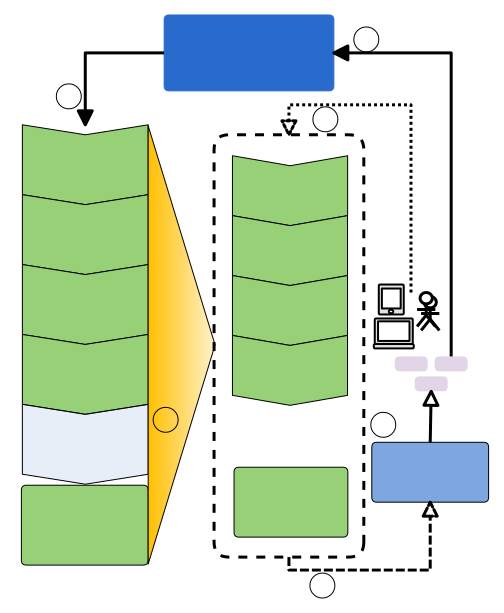
\includegraphics[width=\columnwidth]{../images/motivational-example-vertical.pdf}
\caption{Example Application: Ads Serving}
\label{fig:motivational-example}
\end{figure}

\textbf{Example Application.} 
Online advertising is a multi-billion dollar industry.
An advertising network receives ads from different businesses (ad providers) and shows them on different websites (publishers).
The advertising network charges businesses based on the number of clicks users make on their published ads.
Advertising networks utilize machine learning pipelines to estimate the click rate of different ads.
Figure \ref{fig:motivational-example} shows the workflow of an advertising firm.
The input data (Click Log) consists of several numerical and categorical variables related to the user, the publisher's website, the ads, and whether or not the users clicked on the ads.
A basic click rate prediction pipeline is designed the following way \textcircled{1}. 
A \textbf{missing value imputer} replaces missing values with appropriate values.
A \textbf{string indexer} finds the different unique values in a categorical feature. 
A \textbf{one-hot encoder} creates a new binary feature for every unique value in a categorical feature.
%A \textbf{data bucketizer} transforms continuous variables into a series of binary variables.
A \textbf{standard scaler} scales the data columns to have unit standard deviation and zero mean.
And finally a \textbf{model trainer} trains a logistic regression model over the processed data.
Once the pipeline is created, the deployment platform serves the pipeline and model and prepares them for receiving prediction queries \textcircled{2}.
Whenever a user visits a publisher website, a series of prediction queries are sent to the deployment platform \textcircled{3} .
The deployment platform uses the pipeline to process the request and the model to estimate the click rate of the user for the available ads on the website \textcircled{4}.
An ads selector unit shows the ads with the highest click rate estimates to the user \textcircled{5}.
Depending on whether the user clicks on the ad or not, the platform generates new training data \textcircled{6}.
The deployment platform appends the new training data to the existing click log.
Moreover, new users, ads, and websites may become available while the model is being served.
Therefore, the deployment platform periodically (typically on a daily basis) reprocess the entire data in the click log using the pipeline and trains a new logistic regression model.

The example above demonstrates the complex workflow of a deployment platform.
The deployment platform must be able to guarantee predictions with high accuracy and low latency.
This requires the platform to address the trade-off between the model quality and freshness.
Moreover, the deployment platform must accommodate all the prediction requests and the new training data arriving at the system. 
Our goal is to design a deployment platform that can handle such traffic, provide more accurate predictions to the end user, and provide a balance between model quality and model freshness.

\textbf{Existing Deployment Methods.} 
To ensure accurate predictions, new models should be trained frequently.
However, existing solutions recognize training new models as a resource-intensive and time-consuming process \cite{crankshaw2014missing, agarwal2014laser, baylor2017tfx}.
To address the trade-off between model quality and model freshness, existing solutions propose periodical training of new models.
However, the periods between each instance of the training are typically long (e.g., daily).
While daily training is appropriate for some use cases, it is not suitable for use cases that are required to react quickly to changes in the data (e.g., credit card fraud detection).
This leads to high quality but out-dated models that do not consider the recent training data when answering predictions.
Moreover, existing solutions treat the model training and model serving as two separate processes. 
New models are fully trained in isolation then they are pushed to the deployment environment.

By merging these two processes (training and serving), the training process of new models can be optimized.
In this paper, we propose a method for a deployment platform that continuously updates the models (thus providing fresh models) without sacrificing the quality.
Our solution offers two key optimizations.

\textit{Proactive training.}
Stochastic Gradient Descent (SGD) is an iterative optimization algorithm that is commonly used for training machine learning models on large datasets.
We use SGD to continuously update the deployed model.
Individual iterations of SGD are independent and typically lightweight.
By exploiting these two features of SGD, we replace the time-consuming and resource-intensive training of the new model by a series of single iterations of SGD that are executed proactively.
Our strategy in continuously updating the model is similar to how parameter servers train large models \cite{li2014scaling}.
Parameter servers use the Stochastic Gradient Descent optimization method to iteratively compute partial updates and push these updates to the model.
In our solution, we continuously compute the partial updates based on a combination of the existing data and the newly arrived data.
We then propagate the partial updates to the deployed model.
Proactive training increases model freshness without sacrificing the model quality.
Our experiments show that proactive training of the model achieves more accurate predictions over time and requires fewer resources when compared to the full training of new models.

\textit{Online Statistics Computation and Data Materialization}
We compute and update the statistics of the training dataset in real-time while the model is being served. 
The statistics are required to process the data before training the model.
In our motivating example, label indexing, one-hot encoding, 
%data bucketing, 
and standard scaling require statistics in form of the mean, standard deviation, and feature distribution.
Due to the size of the training dataset, computing these statistics every time before training the model is time-consuming which increases the total training time of the new model.
Updating the statistics in real-time requires a minimal amount of resources. 
To compute mean and standard deviation, we need to update the column sum and dataset size.
To index the labels and perform one-hot encoding, we need to perform a lookup (and in case a new categorical variable is detected, an update) in a hash-table. 
After updating the statistics, each pipeline component transforms the data and passes the data to the next component.
When every component updates their statistics the resulting data is materialized and stored on disk.
As a result, we can directly use the materialized data to train a new model and skip the preprocessing steps of the pipeline.

In summary our contributions are:
\begin{itemize}
\item A platform for continuously training deployed machine learning pipelines and models that adapts to the rate of the incoming data and the model quality requirement.
\item Proactive training of the deployed model using a parameter server style approach that frequently updates the model in-place and increases the quality of the model when compared with state of the art.
\item Efficient training of the model by online statistics computation and data materialization, thus guaranteeing the model freshness without sacrificing the model quality.
\end{itemize}

The rest of this paper is organized as follows:
Section \ref{continuous-training-serving} describes the details of our continuous training approach.
In Section \ref{sec:system-architecture}, we introduce the architecture of our deployment system.
In Section \ref{evaluation}, we evaluate the performance of our continuous deployment approach.
Section \ref {related-work} discusses the related work.
Finally, Section \ref{conclusion} presents our conclusion and the future work.

\section{Continuous Training and Serving} \label{continuous-training-serving}
In this section, first, we describe how we utilize the properties of the stochastic gradient descent to implement the proactive training.
Next, we describe the details of the online statistics computation and feature materialization.
Finally, we demonstrate how our deployment platform improves the existing deployment approaches and maintains the quality of the deployed model.

\subsection{Proactive Training} \label{proactive-training}
Proactive training is a replacement for the periodical offline retraining of the deployed model.
In periodical retraining, when the size of the accumulated training data surpasses a predefined threshold, the platform retrains the deployed model.
Contrary to the periodical training, in proactive training, the platform continuously train the deployed model using the incoming and existing historical data.

We take advantage of the iterative nature of SGD in the design of the proactive training.
\todo[inline]{Alireza: Should not we mention we use mini-batch SGD ? Behrouz: I talk about the sampling separately, we can mention we are using mini batch as well but I'm not sure if that is required}
The input to each iteration of SGD is the current weight parameters of the model, one or more data points, and an objective function.
In proactive training, we execute iterations of SGD on the deployed model.
To execute the proactive training, the deployment platform first samples the historical data.
Then the platform transforms the data into a set of features using the deployed pipeline.
\todo[inline]{Alireza: should not be plural ? Behrouz: I think singular makes more sense, the gradient itself is multi dimensional but the word 'gradient' should be singular. I ll google a bit to see which one's better.}
Next, the proactive trainer utilizes the transformed features to compute the gradient of the objective function.
Finally, the deployment platform updates the deployed model with the computed gradient.

The learning rate parameter of SGD has a significant impact on the proactive training.
To effectively update the deployed model, one has to tune the learning rate.
Similar to the offline SGD, using a constant or decreasing value for the learning rate results in suboptimal training.
Adaptive learning rate methods work well in a dynamic environment where the distribution of the data may change over time \cite{zeiler2012adadelta}.
Therefore, in proactive training, instead of using simple learning rate tuning, we utilize the more advanced learning rate adaptation methods.
The performance of learning rate adaptation techniques varies across different datasets.
To choose the most promising adaptation technique, we rely on hyperparameter tuning during the initial model training on the historical dataset \cite{bergstra2012random}.
After the initial training, the deployment platform utilizes the same learning rate adaptation technique for the proactive training.
\todo[inline]{Alireza: One question which could be raised is : do you compare it with something non-adaptive? Because we use adjective "highest". In general, the satement has to be backed up with experiment. I know we discussed this before (choosing it adaptively and reason for not doing it). Now, the concern is to write it in such a way that does not raise any flag.    Behrouz: The referenced literature show that these adaptation techniques work better than vanilla one, it's true that someone can always ask about it, but just referencing the literature should be enough. Isn't it?}
Our experiments in Section \ref{evaluation} show that selecting the adaptation technique based on initial training results in a model with the highest quality during the proactive training.

\todo[inline]{Alireza: Not sure of usage of modal. Why not just saying it without adding any doubts? Behrouz: Here I wanted to say that because it has to adapt the deployed model, then one has to consider the effect the historical data sampling.}
The proactive training must adapt the deployed model to the recent data items.
As a result, when sampling the historical data, one has to consider the effect of the sample on the deployed model.
A time-based sampling approach of the historical data emphasizes the more recent data points and adapts the deployed model to the changes in the data distribution.
In Section \ref{evaluation}, we evaluate the quality of the deployed model when different sampling techniques are utilized (time-based, uniform, and window-based).
We show that the time-based sampling results in a model with better quality.

%\textit{Model Stability}
%To ensure that proactive training does not degrade the quality of the model, a model evaluator is used to assess the quality of the model.
%The proactive trainer uses the latest deployed model as an initial starting point and updates the model based on the training data.
%The evaluator assesses the quality of the model using an evaluation dataset or the prequential evaluation method \cite{dawid1984present}.
%If the quality of the model has degraded, the update is discard and the model is logged.
%This is to avoid over training the deployed model in proactive training.

%\todo[inline]{I'm going to remove scheduling rate and just run proactive training when the sample buffer is full}
%\textit{Scheduling rate.}
%\hl{An extra parameter of proactive training is the scheduling rate.
%In offline training, iterations of SGD are executed one after the other until convergence.
%In proactive training, the scheduling rate defines the frequency of SGD iteration execution.
%The scheduling rate plays an important role as it directly affects the freshness of the deployed model.
%However, a high scheduling rate results in many frequent SGD iterations which incur an overhead on the deployment system as it is using a lot of resources.
%A small scheduling rate also affects the model freshness.
%To increase the efficiency of the system a scheduler component is designed that is tasked with scheduling new iterations of SGD.
%Similar to learning rate tuning, we use an adaptive approach to adjust the scheduling rate.
%We describe a method for tuning the scheduling rate based on the rate of the incoming training data.
%The scheduling rate is increased as the rate of the incoming training data increases and vice versa.
%This helps in adapting the model to the new training data.}

\subsection{Online Statistics Computation and Feature Materialization}
Before applying the proactive training, the deployment platform needs to transform the data using the deployed pipeline.
Some components of the machine learning pipeline, such as the standard scaler or the one-hot encoder, require statistics over the dataset to be calculated before they process the data.
Computing these statistics require scans of the data.
In our deployment platform, we utilize online training as well as proactive training.
During the online update of the deployed model, we compute all the necessary statistics for every component.
Online computation of the required statistics eliminates the need to recompute the statistics during the proactive training.

Moreover, during the online learning, the deployed pipeline transforms the incoming data to a set of features before updating the model.
Given enough storage space, our deployment platform first assigns timestamps and then caches these preprocessed features.
Therefore, while performing the proactive training, instead of sampling from the raw historical data, the deployment platform samples the features directly from the cache.
Caching the features eliminates the data preprocessing part of the pipeline during the proactive training and significantly reduces the total training time for the proactive training.

\textit{Dynamic model size.}
Some components of the machine learning pipeline generate new features.
For example, one-hot encoding and data bucketization, both may generate new features after processing new training data.
When such components exist in the deployed pipeline, the deployment platform keeps track of the number of features after the data preprocessing.
When the pipeline generates new features, the deployment platform adjusts the size of the deployed model.

\subsection{Improved Deployment Process}
\begin{figure*}[t]
\begin{subfigure}{\columnwidth}
\centering
\includegraphics[width=\columnwidth]{../images/generic-motivational-example-v2.pdf}
\caption{Periodical deployment of machine learning pipelines}
\label{fig:motivational-example}
\end{subfigure}%
\begin{subfigure}{\columnwidth}
\centering
\includegraphics[width=\columnwidth]{../images/generic-improved-example-v2.pdf}
\caption{Continuous deployment of machine learning applications}
\label{fig:improved-example}
\end{subfigure}
\end{figure*}

Figure \ref{fig:motivational-example} shows the process of the periodical deployment approach.
During the initial training, a user designs a machine learning pipeline that consists of several data and feature preprocessing steps. After the data preprocessing step, the user trains a machine learning model by utilizing a batch training algorithm.
During the deployment step, the user deploys the model and the pipeline into the deployment platform.
To perform inference, the deployment platform directs the incoming prediction queries through the preprocessing steps before utilizing the model to predict the label.
During the online update step, the deployment platform directs the training data through the preprocessing steps of the pipeline and then, using an online training algorithm, the platform updates the model.
Finally, the deployment platform accommodates periodical retraining of the pipeline by either automatically initiating a batch training or prompting the user to train and redeploy a new model to the deployment platform.
During the periodical retraining, the deployment platform has to disable the online updating of the model.

Figure \ref{fig:improved-example} shows how our continuous training approach improves the existing deployment process.
Similar to the current deployment process, a user first trains a pipeline and deploy it into the deployment platform.
The deployment platform uses the deployed pipeline and model to answer prediction queries and update the model using the incoming training data.
After transforming the incoming data into a set of features, the deployment platform caches the transformed features.
During the proactive training, the platform samples the cached features and computes the gradient using the sample.
Finally, the platform updates the deployed model using the gradient.
In the new deployment approach, the platform continuously updates the pipeline and the deployed model without requiring full retraining over historical data.
As a result, the deployment platform ensures the model is always up-to-date.
\section{System Architecture} \label{sec:system-architecutre}
Our proposed deployment platform comprises four components; pipeline manager, data manager, scheduler, and SGD runner.
Figure \ref{fig:system-architecture} gives an overview of the architecture of our system and the interactions among its components.

\begin{figure}[t]
\centering
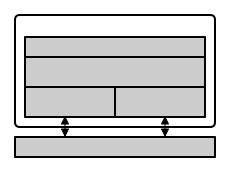
\includegraphics[width=\columnwidth]{../images/system-architecture.pdf}
\caption{System Architecture}
\label{fig:system-architecture}
\end{figure}

\subsection{Scheduler}\label{scheduler}
The scheduler component is responsible for scheduling new iterations of SGD.
The scheduler communicates with pipeline manager to instruct when to execute a new iteration of SGD.
The scheduler allows for two types of scheduling mechanism, namely \textit{static} and \textit{dynamic}.

The static scheduling uses a user-defined parameter that specifies the interval between executions of each iteration of SGD.
This is a simple yet useful mechanism for use cases that require periodical updates of the model when the interval is known a priori (for example, every minute or hour). 
The dynamic scheduling tunes the scheduling interval based on the rate of the incoming prediction, prediction latency, and the time that it takes to execute an iteration of SGD.
The scheduler uses the following formula to computes the time when to execute the next iteration of SGD:

\begin{center}
$T' = (2 * T * pr * pl) / pn$
\end{center}
where $T'$ indicates the time in second when the next iteration is scheduled to run, $T$ is the execution time of the last SGD iterations, $pl$ and $pr$ are the average prediction latency and number of prediction requests per second, and $pn$ indicates the number of parallel instances of the query answering component.
$T$ is measured by the scheduler component itself while $pr$ and $pl$ are measured by the deployment platform.
$pn$ is determined by the underlying execution engine.
Using the formula to schedule the next SGD iteration, the scheduler \hl{guarantees} that all the prediction requests that may arrive while the current SGD iteration is being executed and new prediction requests are answer before a new iteration is scheduled.
\hl{There still some limitations: the execution engine should guarantee that the latency is not prediction answering latency is not greater than 1 second and make sure no more than }
Moreover, the scheduler assumes that the entire resources of the computing cluster is being used by the SGD iteration and therefore the prediction answering component is completely blocked while the SGD iteration is being executed.
By removing the above assumption, SGD iterations can be scheduled to execute more frequently.

\subsection{Data Manager} \label{data-manager}
The data manager component is responsible for storage of historical data, processing the incoming training data, and providing the SGD run-time with a new batch of training data for every iteration.

Historical data is typically large and may not fit in the memory or disk of a single machine. 
The data manager handles the communication with the underlying storage unit.
When new training data becomes available, the data manager appends the incoming data to the existing historical data.
Moreover, the incoming training data are forwarded to the pipeline manager to update the statistics required by the pipeline components.

When a new iteration of SGD is scheduled to run, the data manager is responsible for providing the batch of training data.
The data manager can provide the next batch of training data in two different modes, namely \textit{sample-then-append} and \textit{append-then-sample}.
In the sample-then-append mode, the new training data that has arrived at the system is stored in an intermediate buffer in the memory.
The historical data is sampled and the resulting data is then combined with the data in the buffer.
The data manager makes the combined data available for the SGD run-time to execute the next iteration of SGD.
In the append-then-sample mode, the new training data is appended to the historical data upon arrival.
The data manager then samples the historical data (that consists of the new training data) and provides the resulting dataset for the SGD run-time.

The two operation modes of data manager affect the way the deployed model is evolving over time.
In the sample-then-append mode, every iteration of SGD uses the new training data in its entirety.
Therefore, there is a more emphasis on the recent data than the historical data.
While this is the more desirable method, it may lead to unstable updates, as the distribution of the data may change due to concept drift or anomalies.
Append-then-sample mode assigns the same weight to every data point (new training and the historical data).
As a result, the update to the deployed model is more stable, however, the increase in model quality is smaller than the sample-then-append mode.
In our experiments, we investigate the effect of the different operation mode on model quality and consumption.

%Different sampling strategies can be used to provide the sample.
%In our current prototype, the data manager uses a simple unified random sampling method to generate this sample.
%More advanced methods, such as Reservoir \cite{vitter1985random} or weighted random sampling can also be used to generate the sample.
%Reservoir sampling is typically used to generate samples from large datasets that do not fit in memory, whereas weighted random sampling is used when data elements have different weights.
%In an online machine learning scenario, recent items are more important for training the model and are assigned a bigger weight than older items.
%Therefore, weighted random sampling can generate samples that can contribute to the training of a better model.

Data manager also allows for new training datasets to be registered while the model is being served.
The new dataset is merged with the existing historical data and immediately becomes available for next iterations of SGD.

\subsection{Pipeline Manager} \label{pipeline-manager} 
Pipeline manager is the most important component of the system as it loads the pipeline trained offline, continuously train the pipeline after deployment, evaluate the model update before applying the changes to the deployed model, and exposes the model to answer prediction queries.

Once a pipeline is deployed into the platform, the pipeline manager monitors the pipeline.
The scheduler component informs the pipeline to execute the next SGD iteration.
The pipeline manager then requests the data manager to provide the training dataset for the next SGD iteration.
Once the training dataset is received, the pipeline manager provides the SGD runner component with the current model parameter and training dataset.
Once the SGD iteration is over, the SGD runner sends the updated model back to pipeline manager.
To ensure the quality of the model has not dropped, the pipeline manager uses an independent evaluation set to evaluate the quality of the model.
If the quality of the model does not degrade, the pipeline manager replaces the existing model with the new one.

When new training data arrives at the system, the data manager forwards the data to the pipeline manager. 
The pipeline manager, then, directs the data through the pipeline one component at a time, where each component will receive the data, update their statistics, transform the data and pass it to the next component.
The model training component of the pipeline is skipped as the model is updated separately in SGD iterations.
If the data materialization is enabled, the data processed by the pipeline is sent back to the data manager to be stored with the rest of the materialized data.
Data manager also forwards prediction requests to the pipeline manager.
Similar to training data, the pipeline manager also sends the prediction request through the pipeline to perform the necessary data processing.
Using the same pipeline to process both the training data and prediction requests guarantees that the same set of transformations are applied to both data and prevents inconsistencies between training and serving that is a common problem in model deployment \cite{baylor2017tfx}.
After the prediction request is processed, the pipeline manager uses the model to make a prediction.

\subsection{SGD Runner} 
SGD runner is responsible for executing iterations of SGD.
It is responsible for tuning the learning rate parameter of SGD.
In every iteration, the SGD runner receives a training dataset and the initial model parameter from the pipeline manager, then performs one iteration of SGD and returns the updated the parameter to the pipeline manager.
Although iterations are independent of each other, SGD runner needs to store the necessary information for computing the learning rate for next iterations.
SGD runner is the only component that is tightly coupled with the execution engine as it directly executes the code on the engine.
Therefore, separate implementations have to be provided for the different execution engines.


\subsection{Execution Engine}
All of the components of our deployment platform described so far, except for SGD runner, are decoupled from the execution engine.
In our deployment platform any data processing platform capable of processing data both in batch mode (for continuous training) and streaming mode (answering prediction requests is a suitable execution engine.
Apache Flink \cite{carbone2015apache}, Apache Spark \cite{zaharia2010spark} are distributed data processing platforms can support both stream and batch data processing.
They work with data in memory and on disk which speeds up the execution of SGD iterations.

\textit{Current Prototype}
In our current prototype, we are using Apache Spark \cite{zaharia2010spark} as the execution engine.
The data manager component uses Hadoop Distributed File System (HDFS) for storing the historical data \cite{shvachko2010hadoop}.
We also some components of the machine learning library in spark to implement SGD runner.
To enable real-time prediction answering we use Spark streaming \cite{zaharia2013discretized}.
Spark streaming allows us to define the parallelism parameter ($pn$) and extract prediction requests rate and latency ($pr$ and $pl$).
Job scheduler uses these parameters to schedule new iterations of SGD.

\section{Evaluation} \label{evaluation} 
\todo[inline]{structure is finalized}
In this section we evaluate the performance of our system using various datasets. 
We report both the quality (error rate) and performance of our proposed method. 

\subsection{Setup}\label{subsec:setup}
We evaluate our deployment method in distributed environment consists of 11 nodes (1 master, 10 slaves).
Each node is running on an Intel Xeon 2.40 GHz 16 core processor and has 28 GB of dedicated memory for running our prototype.

To demonstrate the deployment platform designed the following machine learning pipeline.

\textbf{Criteo pipeline.} 
The Criteo pipeline consists of 5 operations: input parser, missing value imputer, standard scaler, one hot encoder, and logistic regression model trainer. 
The Terabyte Criteo click log dataset is used for benchmarking algorithms for clickthrough rate (CTR) prediction \cite{criteo-log}.
It contains 24 days of user click logs. 
The dataset  contains 13 numerical and 26 categorical features. 
In all of our experiments we are using the data from the first 6 days (Day 0 to Day 5) of the Criteo dataset.
Day 0 is used for the initial offline training of the pipeline.
Day 1 to Day 5 are used as a streaming dataset.
To evaluate the quality of the pipeline, we use a sample of the Day 6 to compute the logistic loss.

\subsection{Learning Rate Adaptation Method}
In Section \ref{sgd}, we discussed the importance of learning rate tuning for training a model using the Stochastic Gradient Descent optimization method.
Proactive training is an extension of SGD, therefore the process of tuning the learning rate adaptation method is no different from tuning the it for training.
Figure \ref{fig:criteo-learning-rate} shows the log loss for different learning adaptation methods. 
During the training phase, we evaluated the logistic loss on evaluation dataset after 20, 40, 80, 160, 320, and 500 iterations.
We did not include the results of 
Both Adadelta and Momentum performs very poorly on the criteo data.
Criteo dataset is a complex and high dimensional dataset, where features are a mix of numerical and categorical.
Since categorical features are not standardized, Adadelta and Momentum are not able to effectively tune the learning rate for a mix standardized and non-standardized features.
Both RMSPROP and ADAM manage to effectively reduce the logistic loss during the training phase.
Both methods resulted in the model to converge after 500 iterations.
However, ADAM achieves a lower error rate on the evaluation data when compared to RMSPROP.
After 500 iterations of training, we deploy the pipelines.
We streamed Day 1 of the Criteo dataset to the deployment system and monitored the changes in the loss using the same evaluation dataset.
After deployment, both RMSPROP and Adam further decreased the loss from 0.190 and 0.155 to 0.185 and 0.151 respectively.
Adadelta also reduces the loss by around 0.004, however, the deployed pipeline trained using Adadelta learning rate adaptation technique was not fully converged and as a result the final error rate after the first day is still quite high.
For the rest of our experiments, we chose ADAM as the learning rate adaptation technique.
When using ADAM, the model converges using fewer number of iterations as compared to other learning rate adaptation methods.
Moreover, ADAM is the most effective learning rate for continuous training of the pipeline as well.

\begin{figure}[H]
\includegraphics[width=\columnwidth]{../images/experiment-results/learning-rate-experiment.eps}
\caption{Learning rate adaptation technique for Criteo pipeline}
\label{fig:criteo-learning-rate}
\end{figure}

\subsection{Rate of New Features}
We measure model freshness by two metrics: training recency and rate of new features.
Training recency is determined by the scheduling rate.
Performing more frequent training results in models that can adapt to changes in the data more rapidly.
In Criteo pipeline, we use a feature encoder to transform the categorical features into binary indicator variables.
The initial training data (Day 0) only contains a small portion of all the unique categorical features of the Criteo dataset.
The incoming training data may contain features that have not existed in the dataset before.
Figure \ref{fig:criteo-feature-discovery} shows the feature size overtime for the first 5 days after deployment of Criteo pipeline.
The rate of incoming new features is roughly 30,000 per minute and every day around 45 million new features are generated.
Using our continuous training approach, we update the pipeline as soon as new features become available.
During the next scheduled proactive training, the model is updated using these new features.
As a result, the deployed pipeline is able to answer prediction queries that may contain the same set of features more accurately.
Using a daily training approach, any unseen features that arrive at the system are dropped before a prediction is made.

\begin{figure}[H]
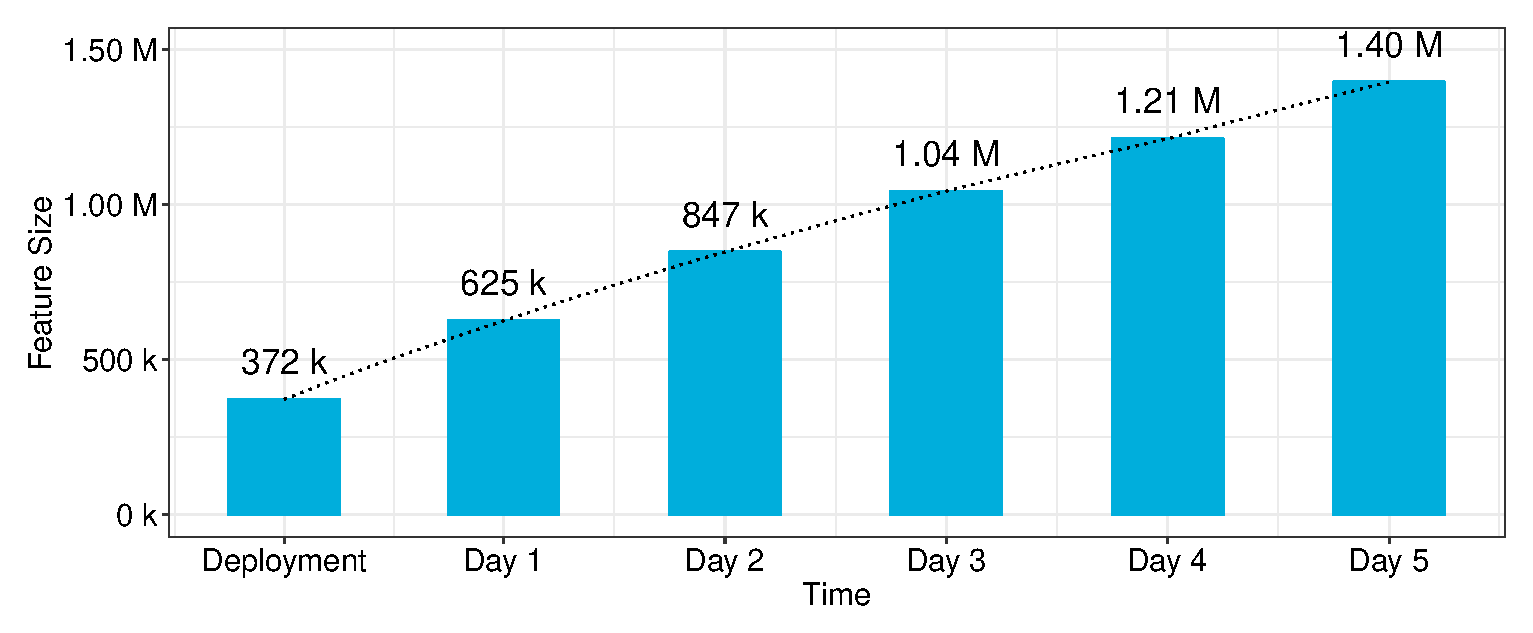
\includegraphics[width=\columnwidth]{../images/experiment-results/feature-discovery-experiment.eps}
\caption{Criteo categorical feature size over time}
\label{fig:criteo-feature-discovery}
\end{figure}

\subsection{Sampling Methods}
\todo[inline]{redo this part, compare weighted time-based sampling vs random sampling different sizes}
In each iteration of SGD the data inside the buffer and a sample of the historical data is combined to update the model.
In this section, we investigate the effect of the sampling rate on the model quality and the running time of the system.
Figure \ref{fig:movie-lens-100k-sample-rate} shows that a larger sampling rate increases the quality of the model.
However, similar to the scheduling rate, the decrease in error rate is negligible considering the effect it has on running time. 
This is caused by the same phenomena, where the model after training on bigger sample rates start to converge faster.
As a result, bigger sample sizes do not have a considerable effect on the quality.
 
Figure \ref{fig:movie-lens-100k-sample-rate-time} shows the effect of increasing the sampling rate on the running time.
Increasing the sampling rate from 0.1 to 1.0, increases the running time by a factor of 5.
\todo[inline]{R3: . The sampling parameter deserves a more systematic treatment since it deeply affects the performance. In fact, Baseline+ and Velox represent two extreme settings of it: 0\% and 100\%. Instead, the paper simply suggests "setting the sampling rate to smaller values will increase the performance substantially, while only slightly affecting the quality of the model." It is not a sound conclusion if we agree Baseline+ is equivalent to 0\% sampling rate.}
Therefore, similar to the scheduling rate, setting the sampling rate to smaller values will increase the performance substantially, while only slightly affecting the quality of the model.

\textbf{Tuning parameters based on error rate:} The underlying machine learning model and the dataset have big effects on the selection of sampling rate and scheduling rate.
In the recommender system use case, due to the changes in the incoming data distribution, we see that bigger sample rates and higher scheduling rates have an effect (although small) on the quality of the model.
However, this is not be the case for every application.
To demonstrate this, we perform the same set of experiments on the MNIST dataset.
Figure \ref{fig:mnist-sample-rate} shows the effect of different sampling rates on the neural network classifier model for MNIST.
Contrary to the results we achieved for Movie Lens 100k, the error rates for different sampling rates are very similar.
This is caused by how neural networks behave.
Increasing the sampling rate causes similar data items to be used repeatedly in consecutive training iterations.
Neural networks are not affected by this oversampling, therefore the results are almost similar with different sampling rates.
Moreover, in this experiment, the number of parameters of the multi-layer perceptron is far less than the number of parameters of the matrix factorization model for Movie Lens 100k.
This causes the neural work to converge faster.
Therefore it is not affected by more training, unless new training observations arrive at the system.

\begin{figure}[h]
\begin{subfigure}{\columnwidth}
\centering
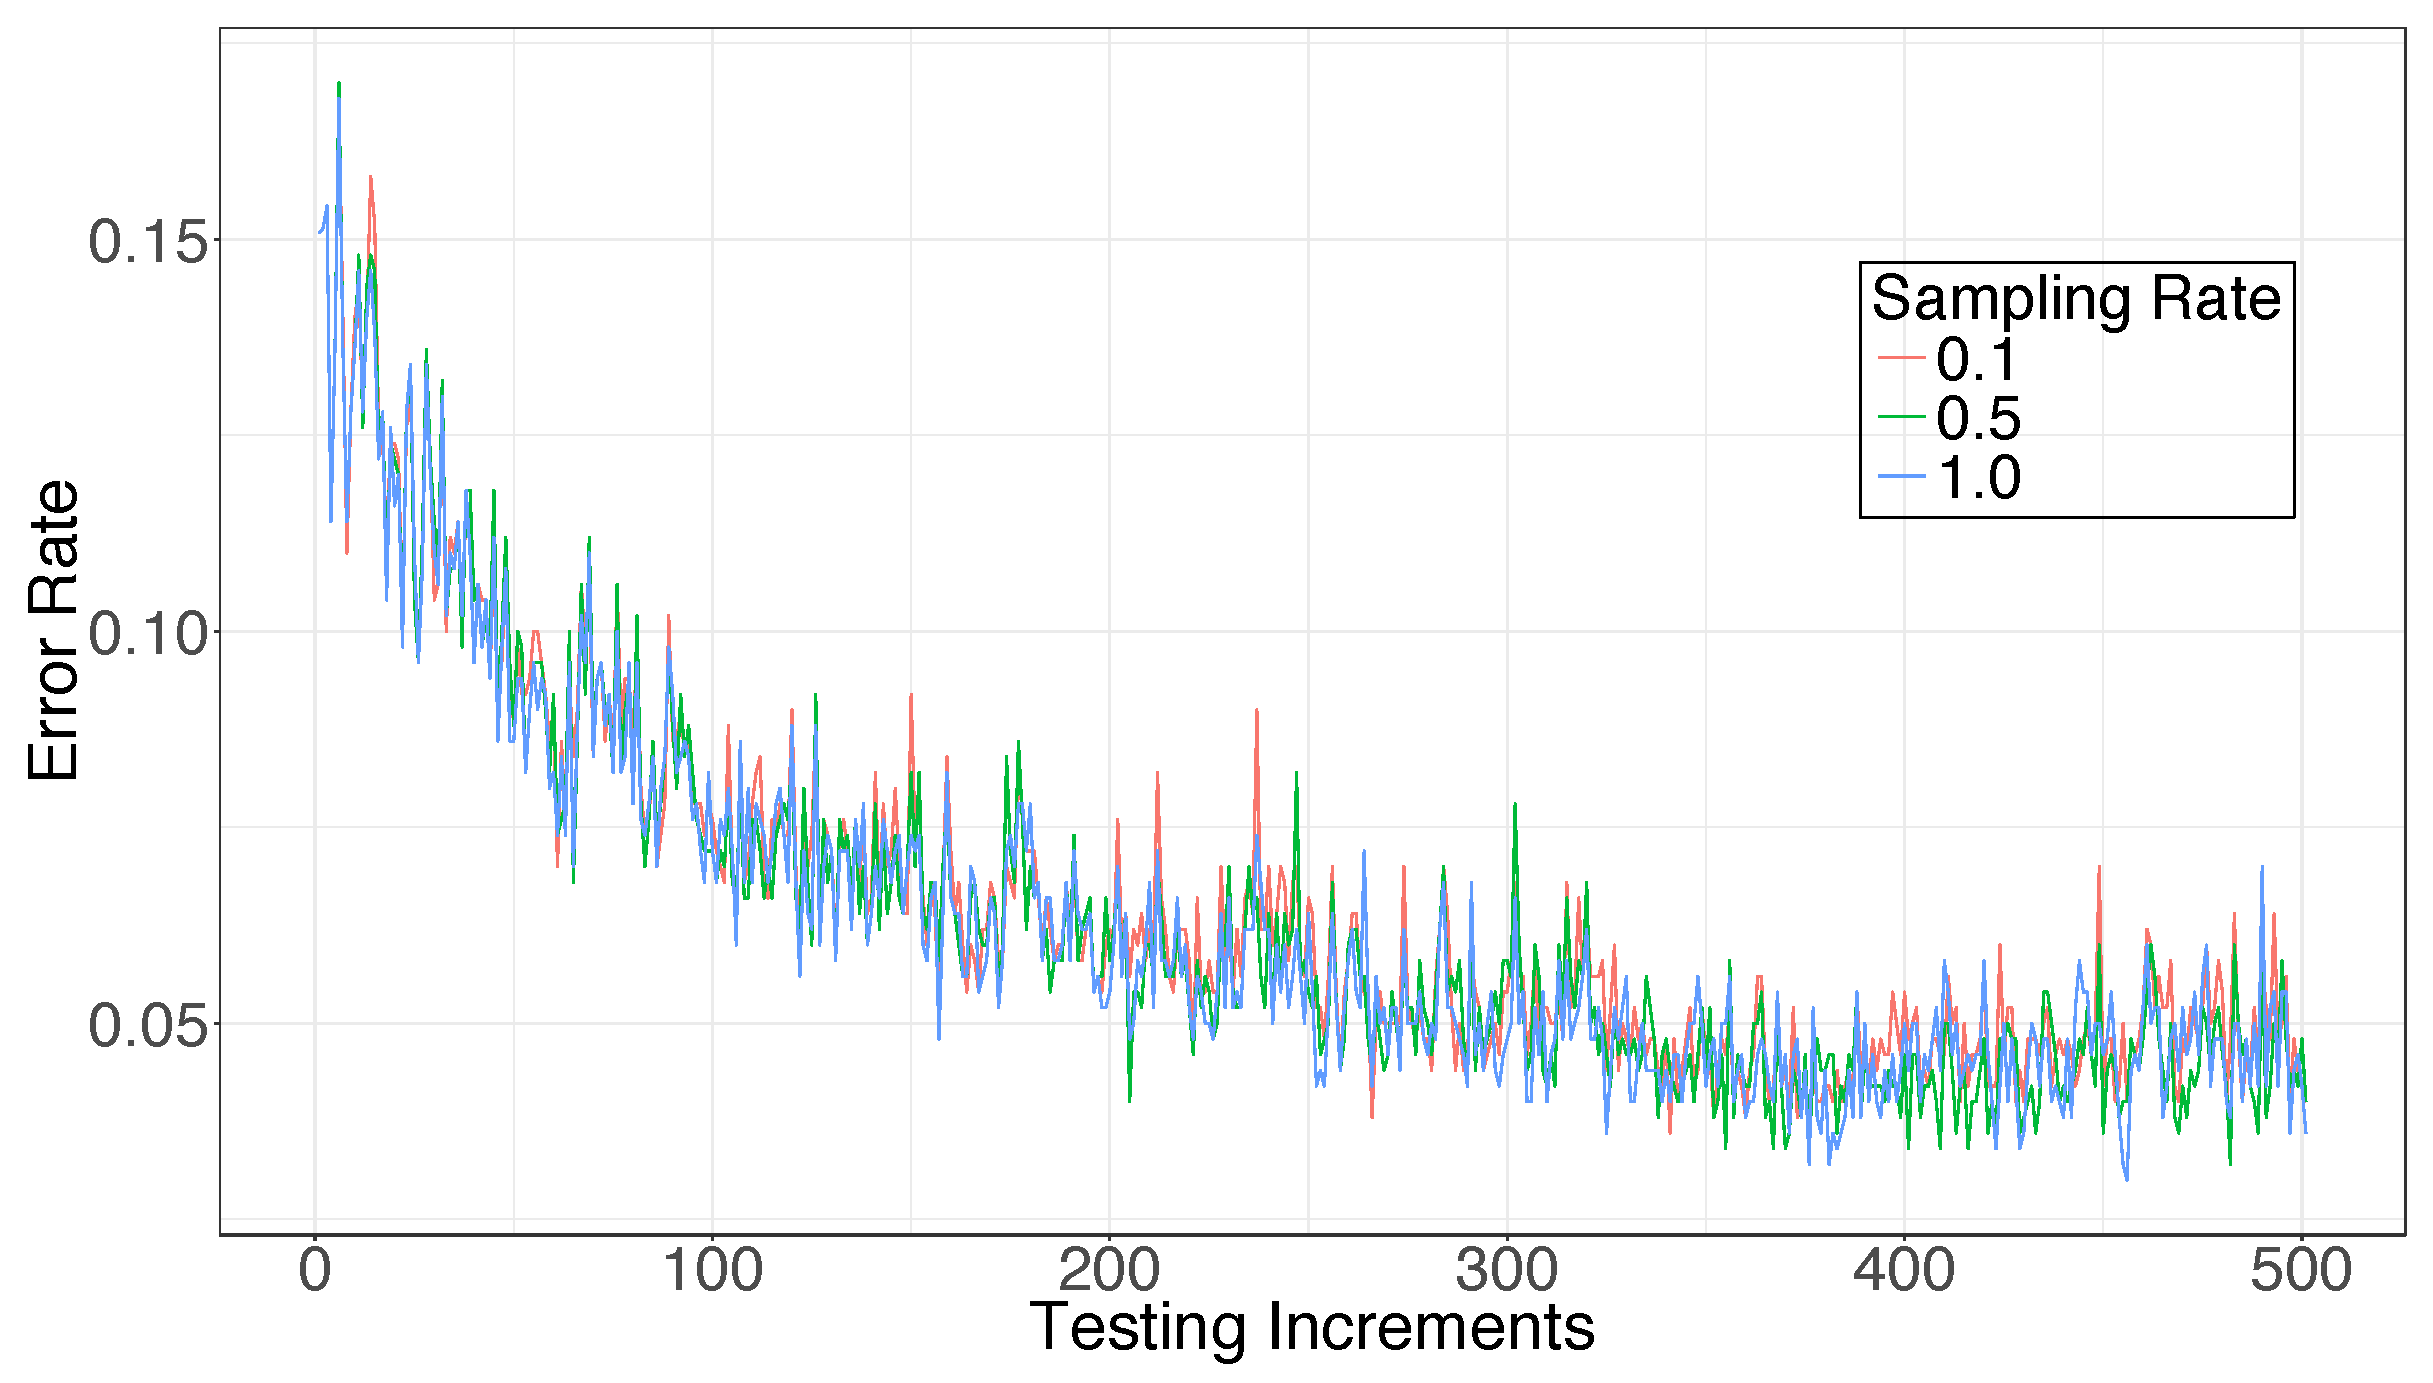
\includegraphics[width=\columnwidth]{../images/experiment-results/mnist-sampling-improved.eps}
\caption{Sampling rate}
\label{fig:mnist-sample-rate}
\end{subfigure}
\begin{subfigure}{\columnwidth}
\centering
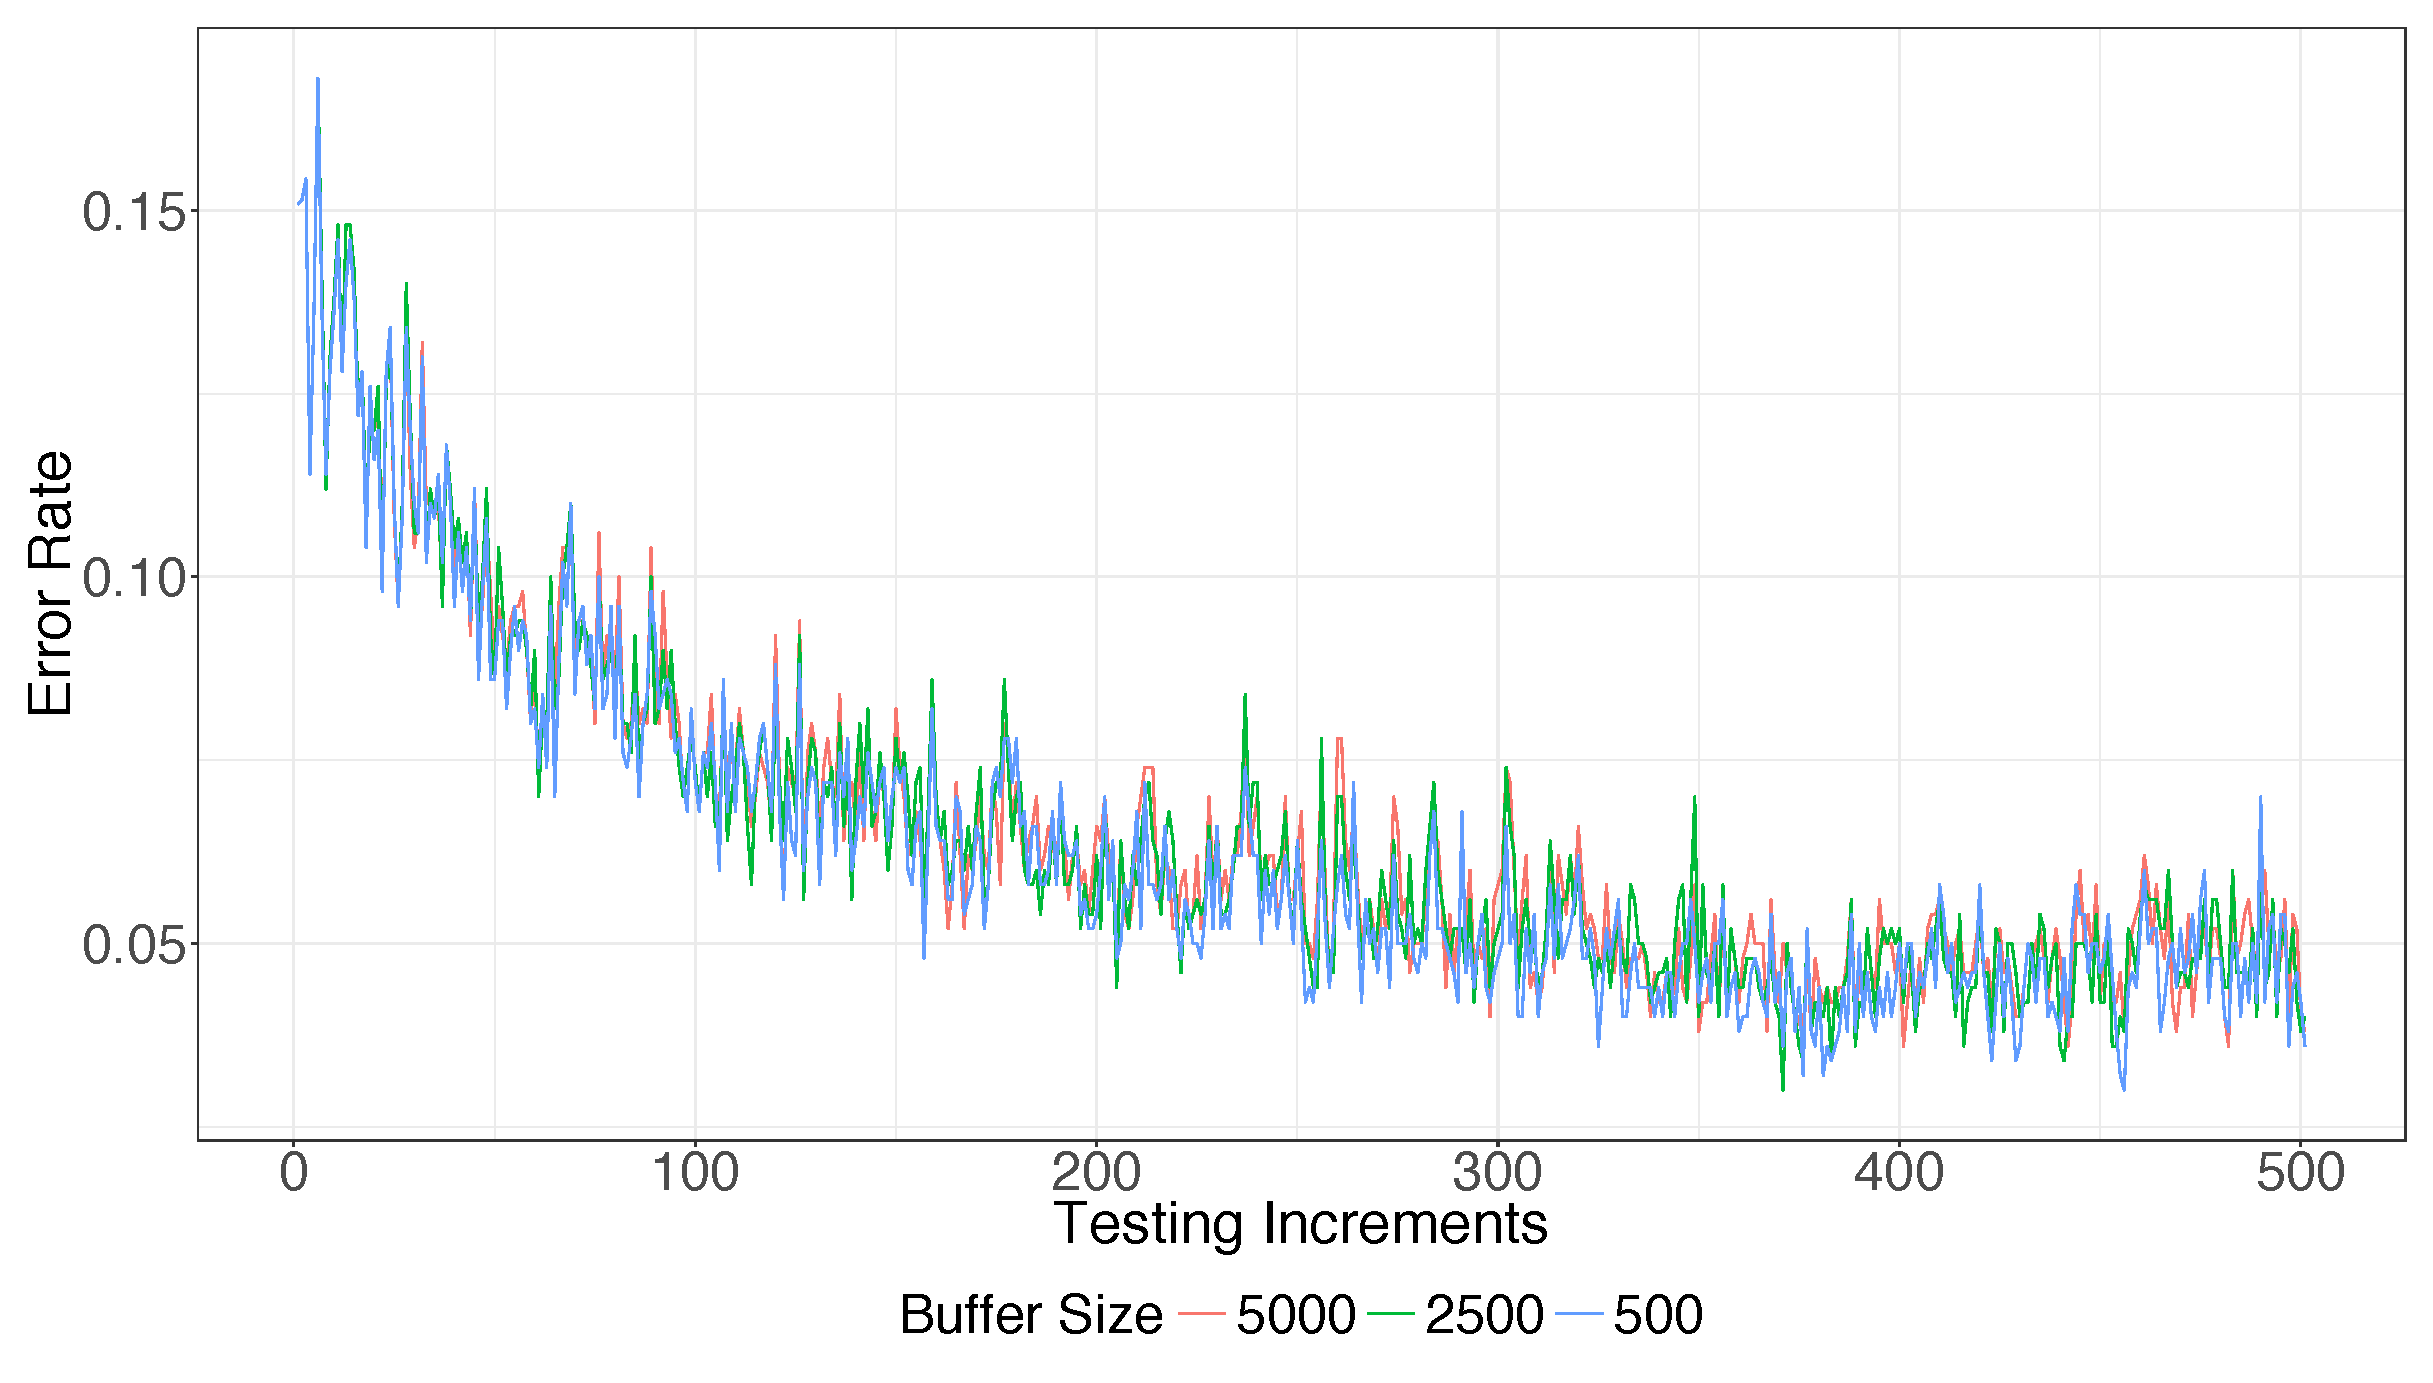
\includegraphics[width=\columnwidth]{../images/experiment-results/mnist-buffersize-improved.eps}
\caption{Buffer size}
\label{fig:mnist-buffer-size}
\end{subfigure}
\vspace{2mm}
\caption{Effect of Sampling and Scheduling Rate on Quality (MNIST)}
\end{figure}

Figure \ref{fig:mnist-buffer-size} shows how the buffer size affects the overall quality of the neural network model.
Similar to the sampling rate case, the error rate of the model is not affected by the scheduling rate.
New training observations that exist in the buffer have the maximum effect on the quality of the model since they are becoming available to the model for the first time.
As the scheduling rate increases, the number of new training observations remain the same, and only the historical data is used more frequently to train the model.
Since neural networks do not gain much benefit by revisiting the same items, increasing the scheduling rate has no effect on the overall quality.

Based on our findings, we conclude that increasing the sampling and scheduling rate does not always affect the quality.
In both the Movie Lens 100k and MNIST datasets, the change in scheduling and sampling rate have small to no effect on the overall quality.
However, the running time of the methods are heavily influenced by these parameters.
\todo[inline]{R3: Similarly, the treatment of buffer size is also shallow. "Setting these parameters to small values decreases the running time considerably and save computation resources regardless of the type of model the system is serving." What about setting the buffer size as 1? BD: Reviewer's confusion is because I have used both scheduling rate and buffer size in the text, although they both control how often a training iteration is executed, they are 'opposite' of each other. Increasing the scheduling rate means we have a smaller buffer size and decreasing the scheduling rate means we have a bigger buffer size. }
Setting these parameters to small values decreases the running time considerably and save computation resources regardless of the type of model the system is serving.

\subsection{Scheduling Policy}
\todo[inline]{redo this part using the criteo dataset}
This parameter specifies how often a new iteration of SGD should be scheduled. 
In our prototype, the scheduling rate is governed by a parameter called buffer size, which dictates how many new items should be stored in the buffer before a new iteration of SGD is executed. 
Executing one iteration of SGD, even using the entire data, is not a resource heavy process, and can be executed simultaneously with the serving component of the system. 

\begin{figure}[h]
\begin{subfigure}{\columnwidth}
\centering
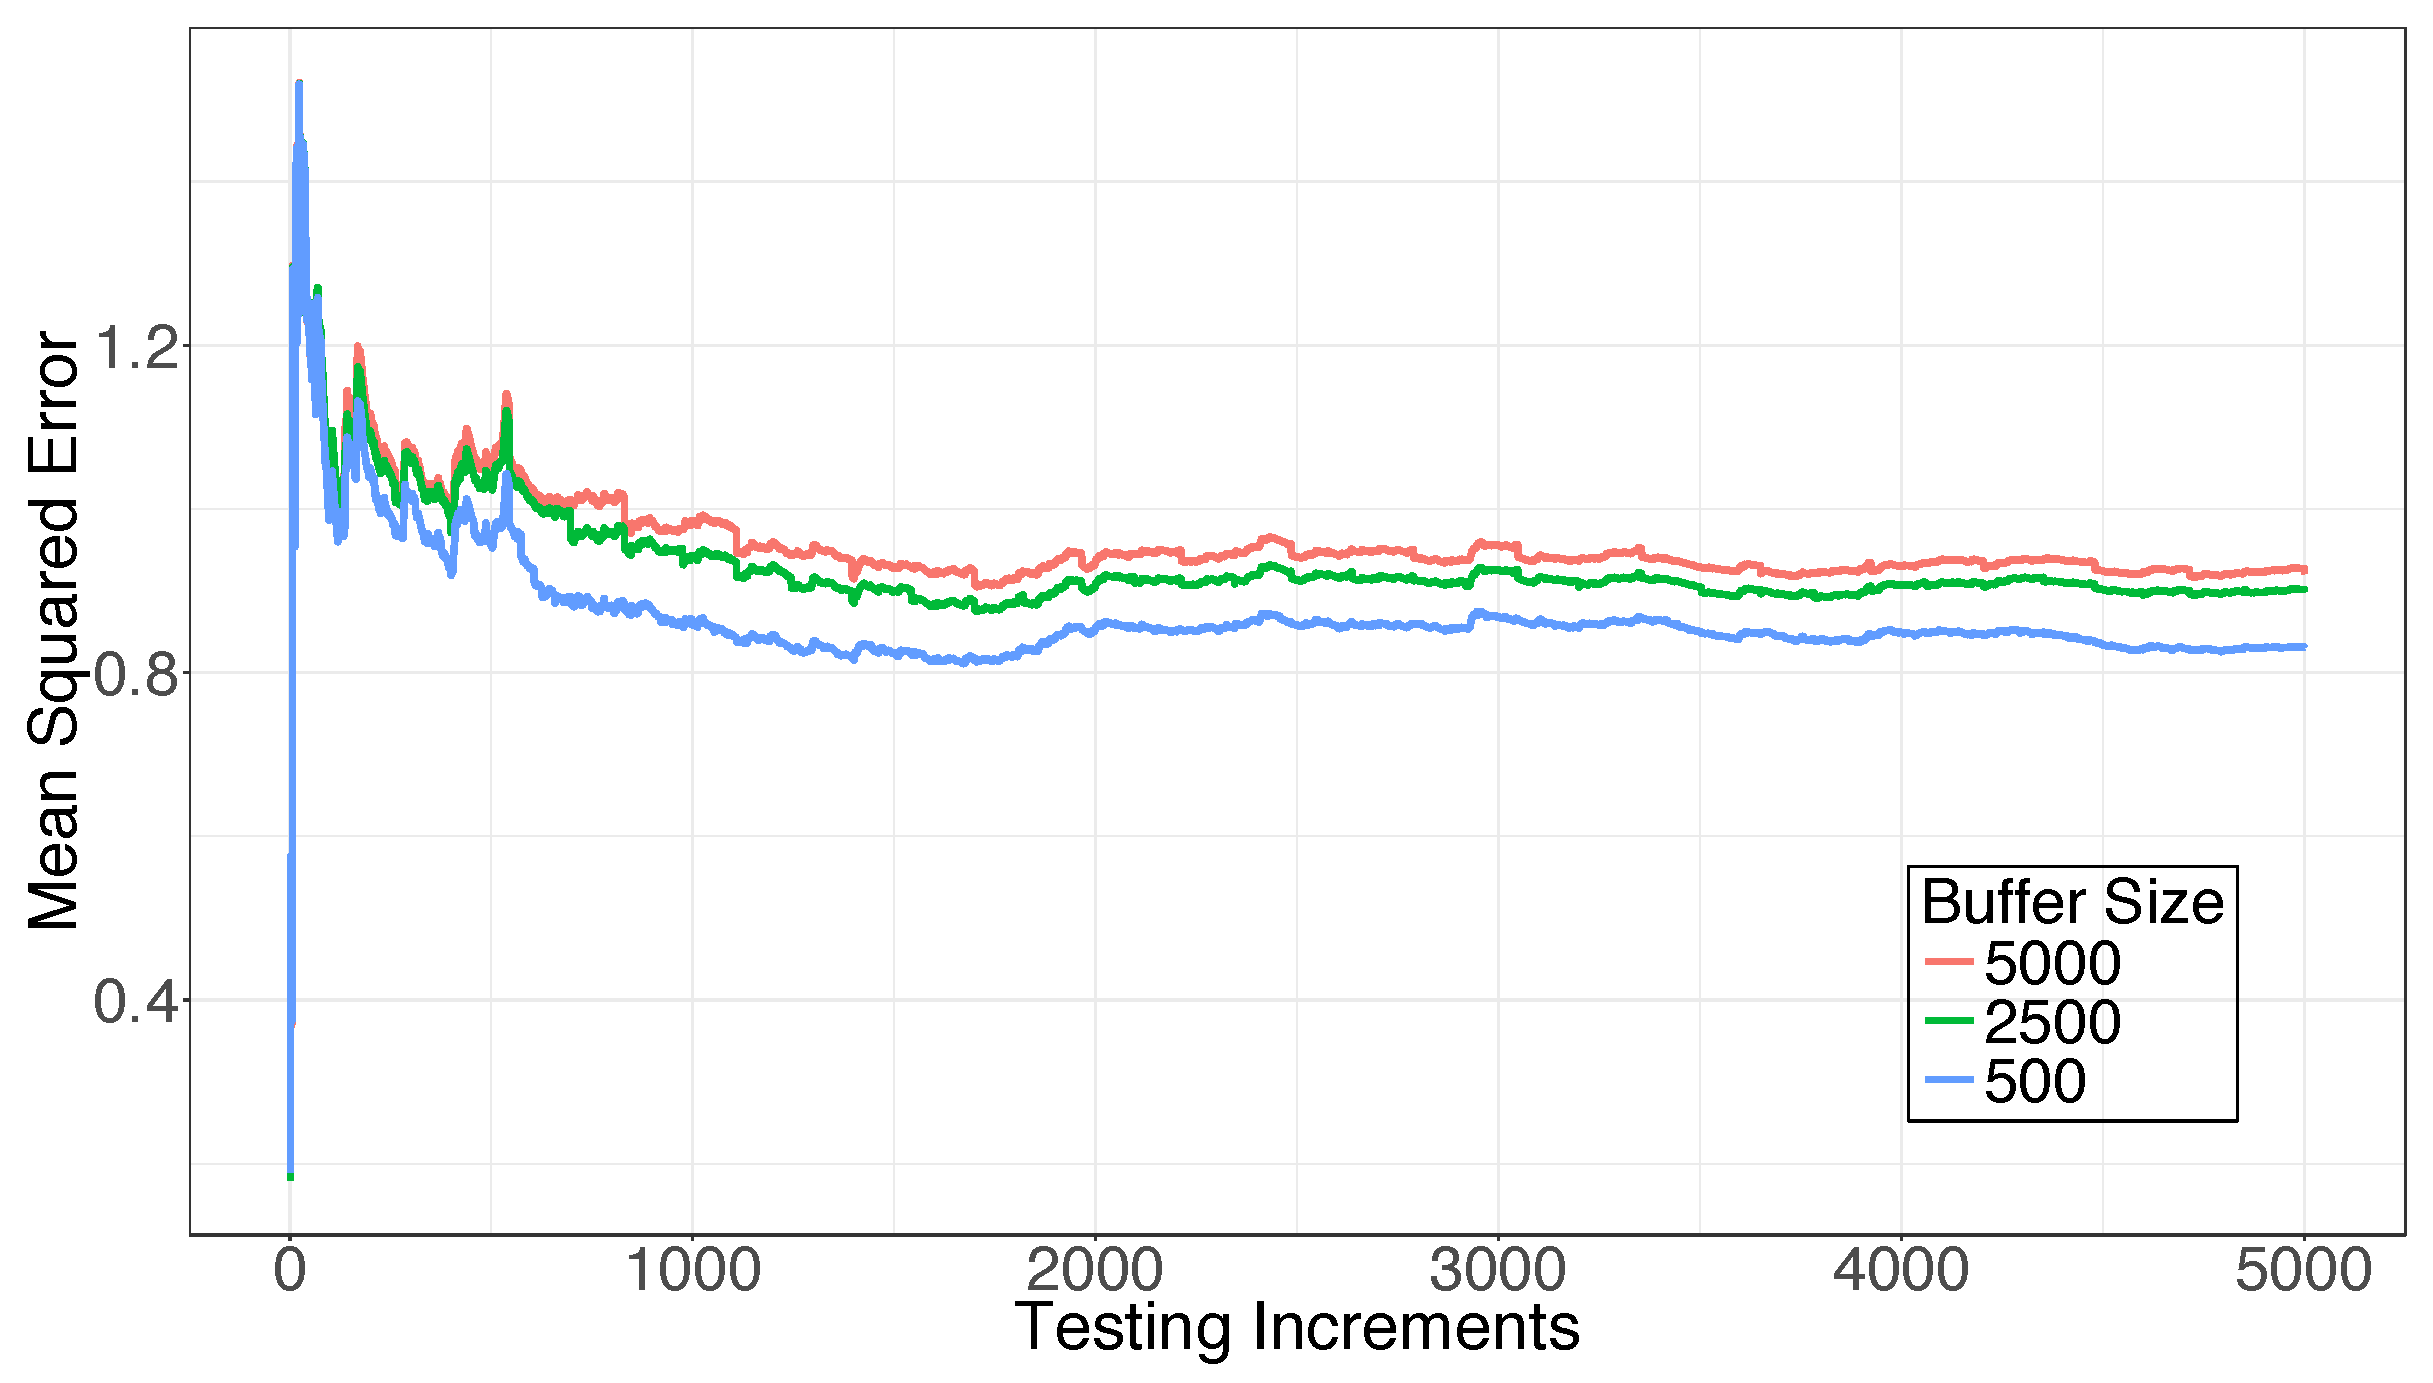
\includegraphics[width=\columnwidth]{../images/experiment-results/movie-lens-buffer-quality-improved.eps}
\caption{Buffer size}
\label{fig:movie-lens-100k-buffer-size-mse}
\end{subfigure}
\begin{subfigure}{\columnwidth}
\centering
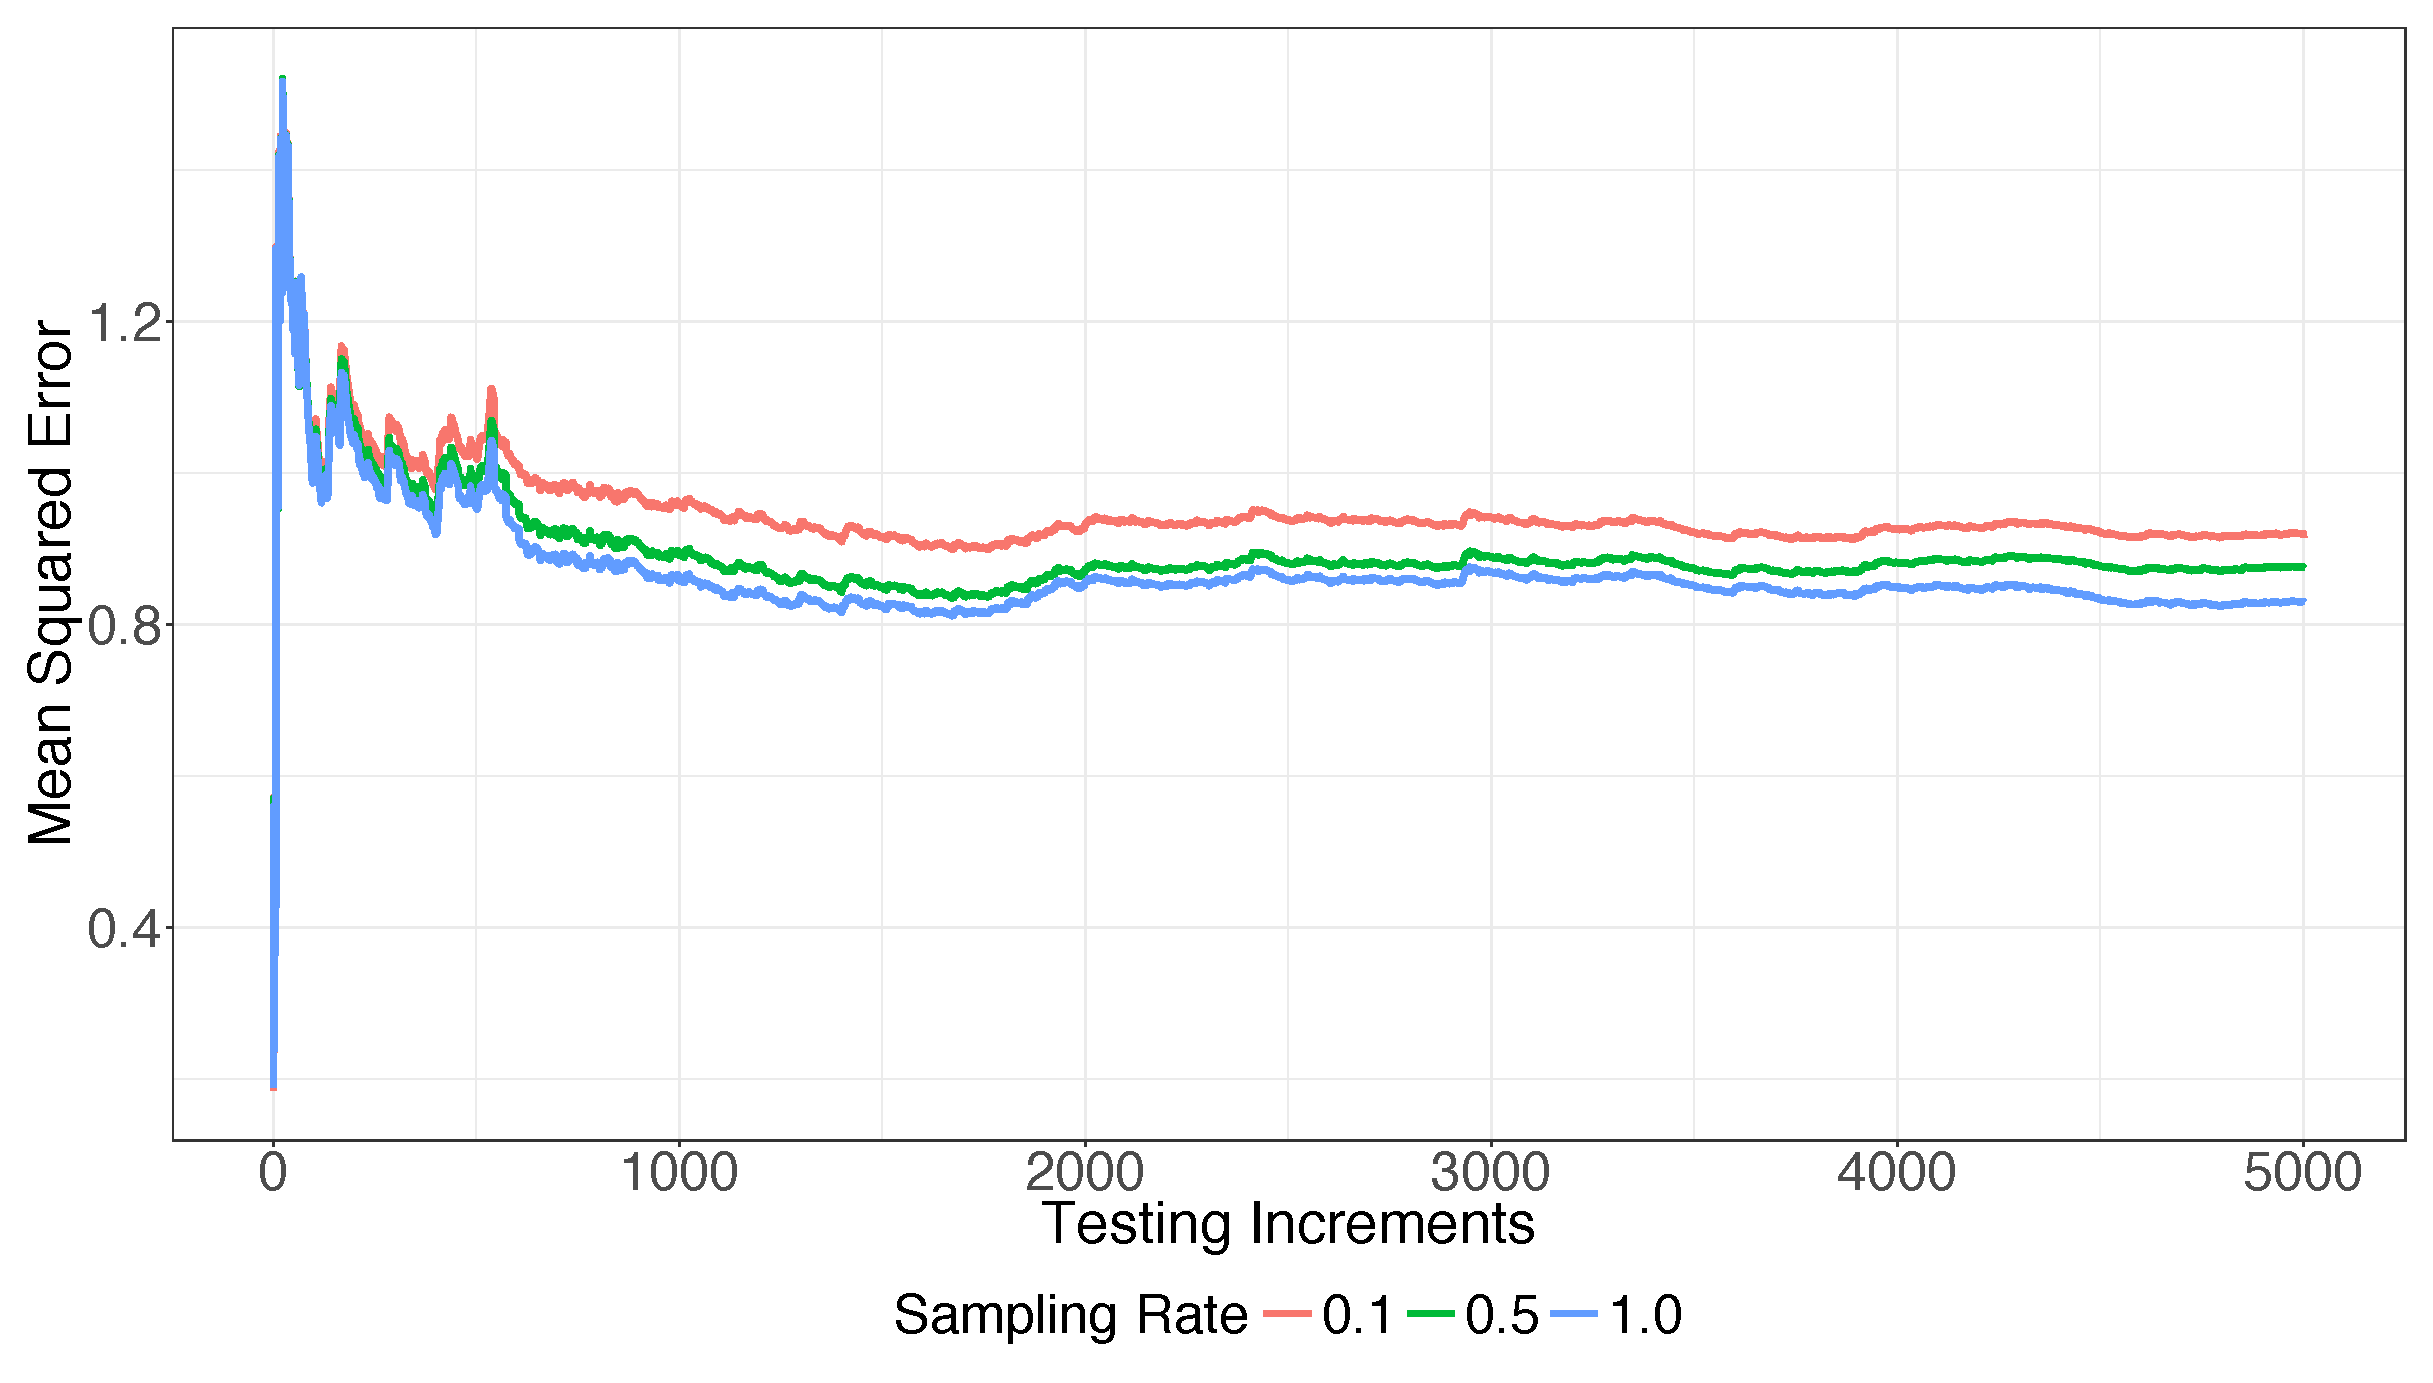
\includegraphics[width=\columnwidth]{../images/experiment-results/movie-lens-sampling-quality-improved.eps}
\caption{Sampling rate}
\label{fig:movie-lens-100k-sample-rate}
\end{subfigure}
\vspace{2mm}
\caption{Effect of Sampling and Scheduling Rate on Quality (Movie Lens 100K)}
\end{figure}

Figure \ref{fig:movie-lens-100k-buffer-size-mse} shows the mean squared error for different buffer sizes for Movie Lens 100k. 
A smaller buffer size forces the scheduler to initiate training iterations more frequently.
As a result, the system updates the underlying model more often.
However, the error rate is not decreasing linearly with the buffer size.
Further analysis shows that the more frequent the model updates are, the faster the model converges and any further training has little to no effect on the overall quality.
This is extremely important, specially when considering the effect of the buffer size on the running time.
Figure \ref{fig:movie-lens-100k-buffer-size-time} shows the running time on Movie Lens 100k using different buffer sizes. 
Increasing the buffer size from 500 to 5000 decreases the running time by a factor of 5 while the MSE is only decreased slightly.
Therefore, depending on the application, we can set the buffer size to bigger values in order to increase the performance of the system without affecting the quality of the final model substantially.

\begin{figure}[H]
\begin{subfigure}{0.5\columnwidth}
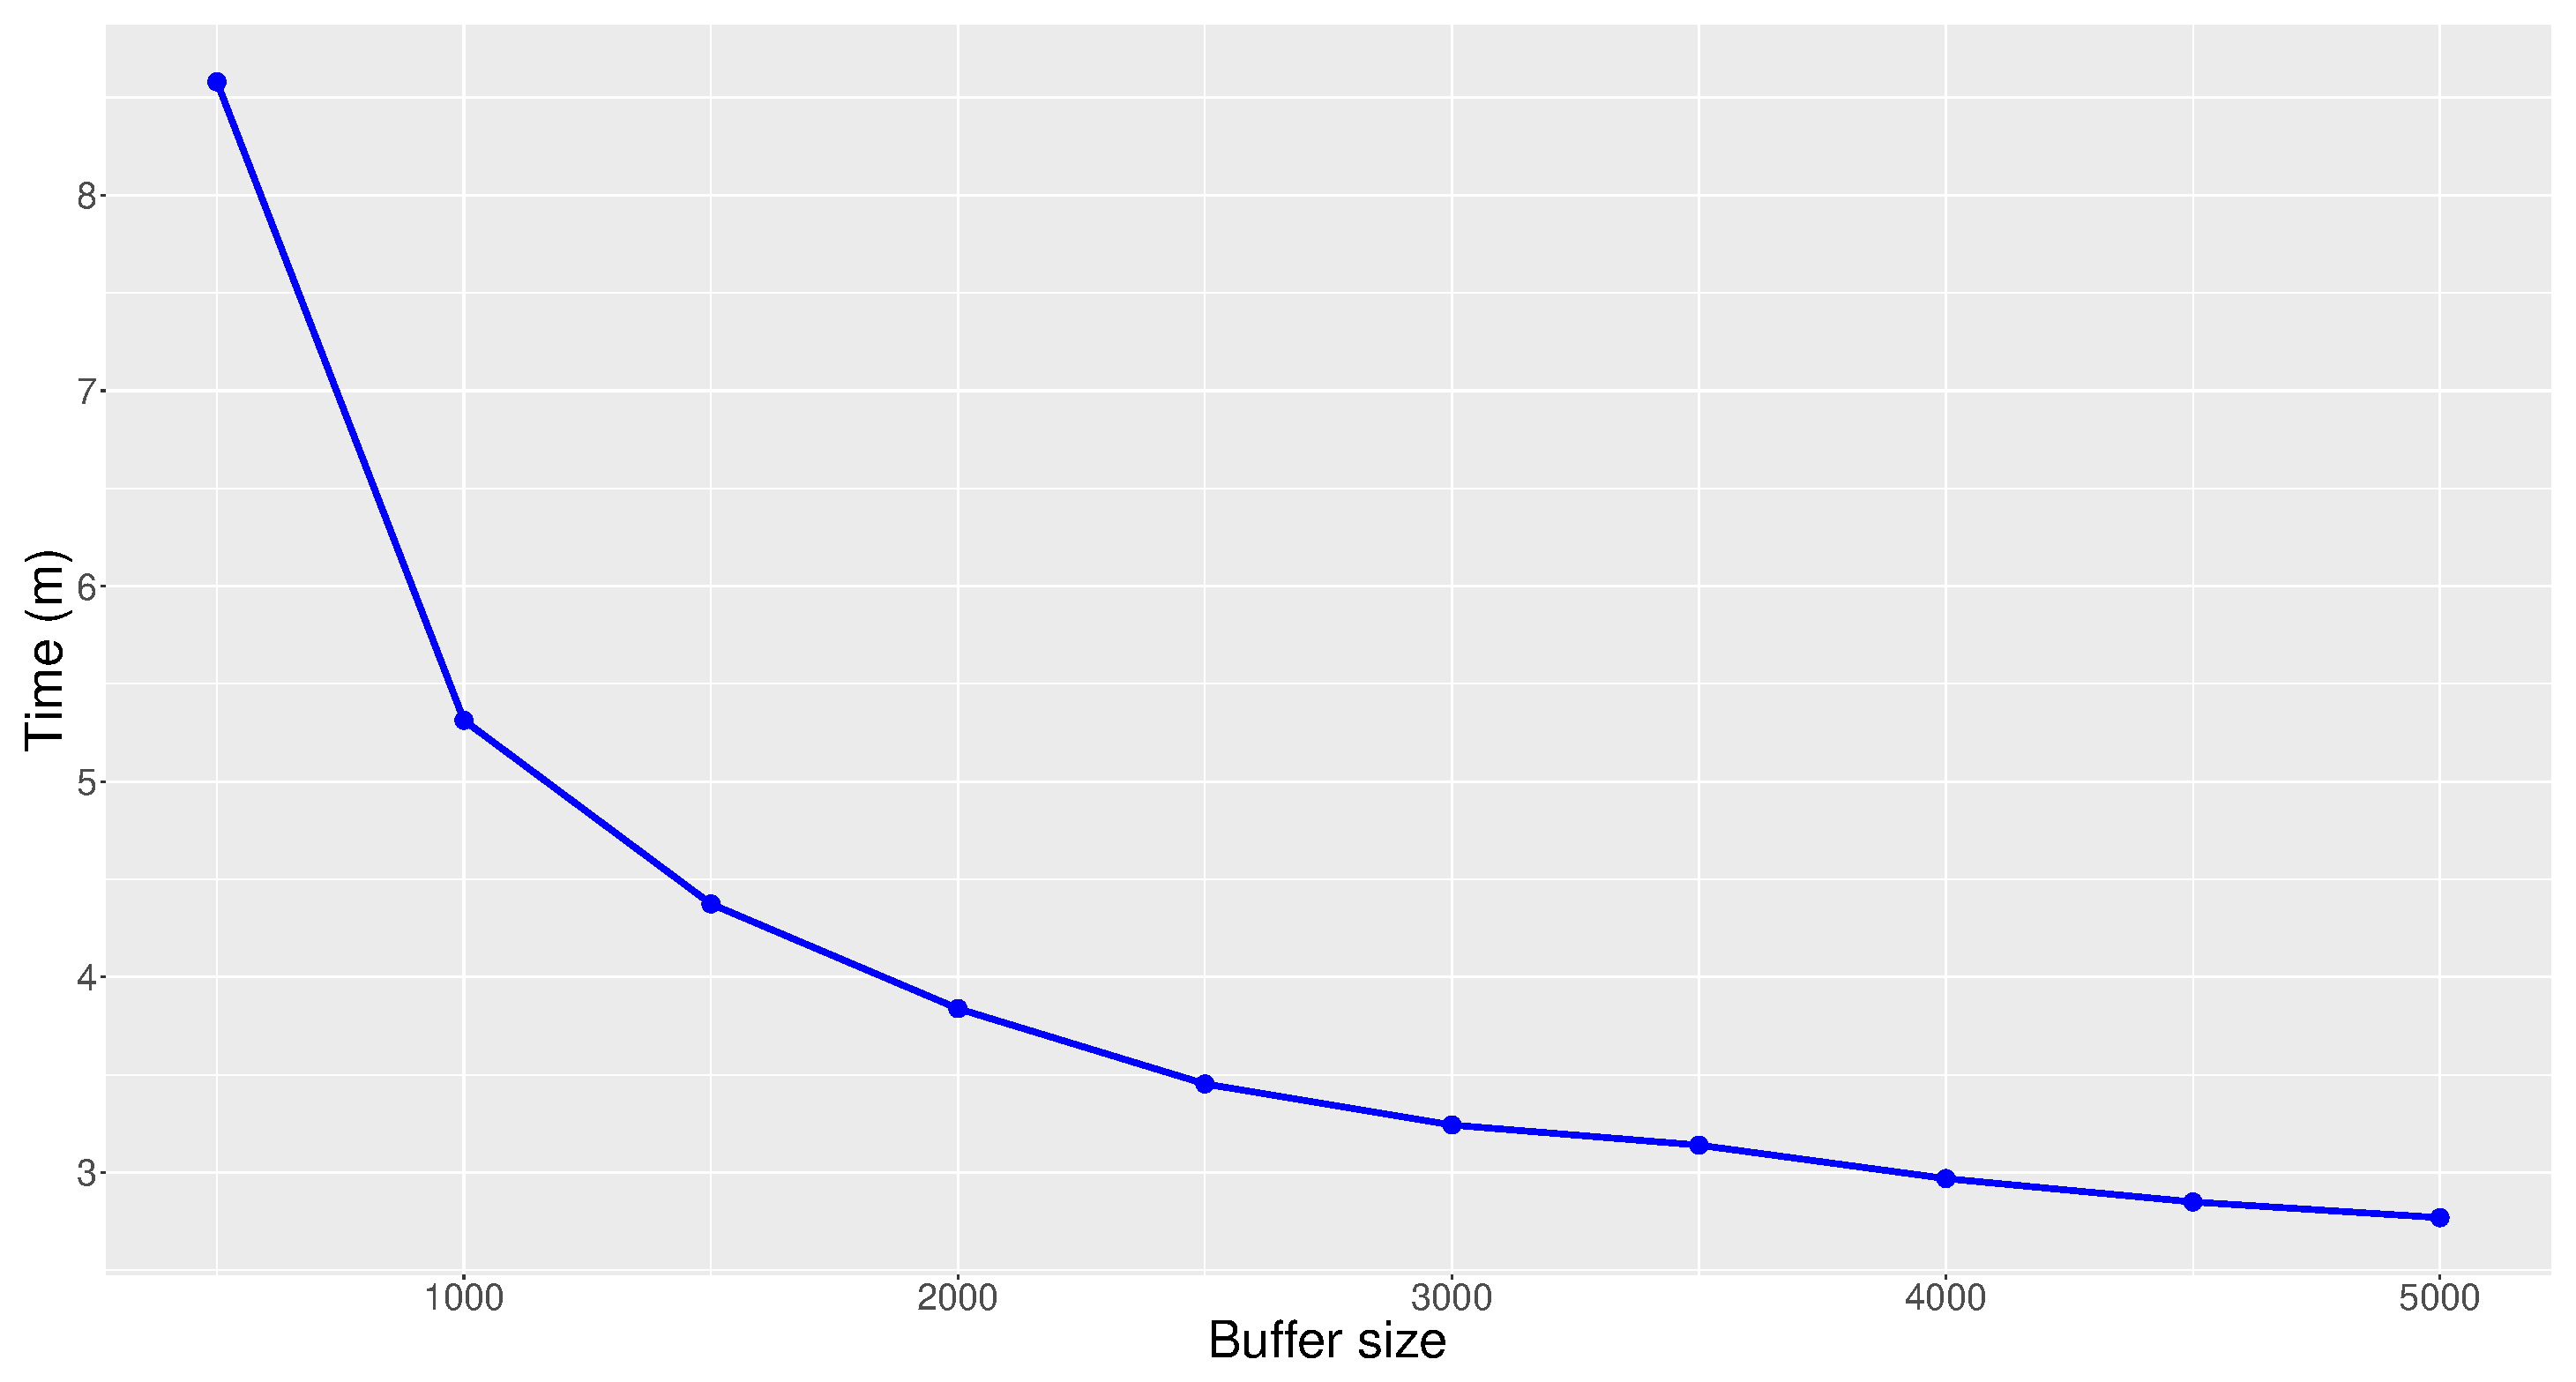
\includegraphics[width=\columnwidth]{../images/experiment-results/movie-lens-100k-buffer-time-improved.eps}
\caption{}
\label{fig:movie-lens-100k-buffer-size-time}
\end{subfigure}%
\begin{subfigure}{0.5\columnwidth}
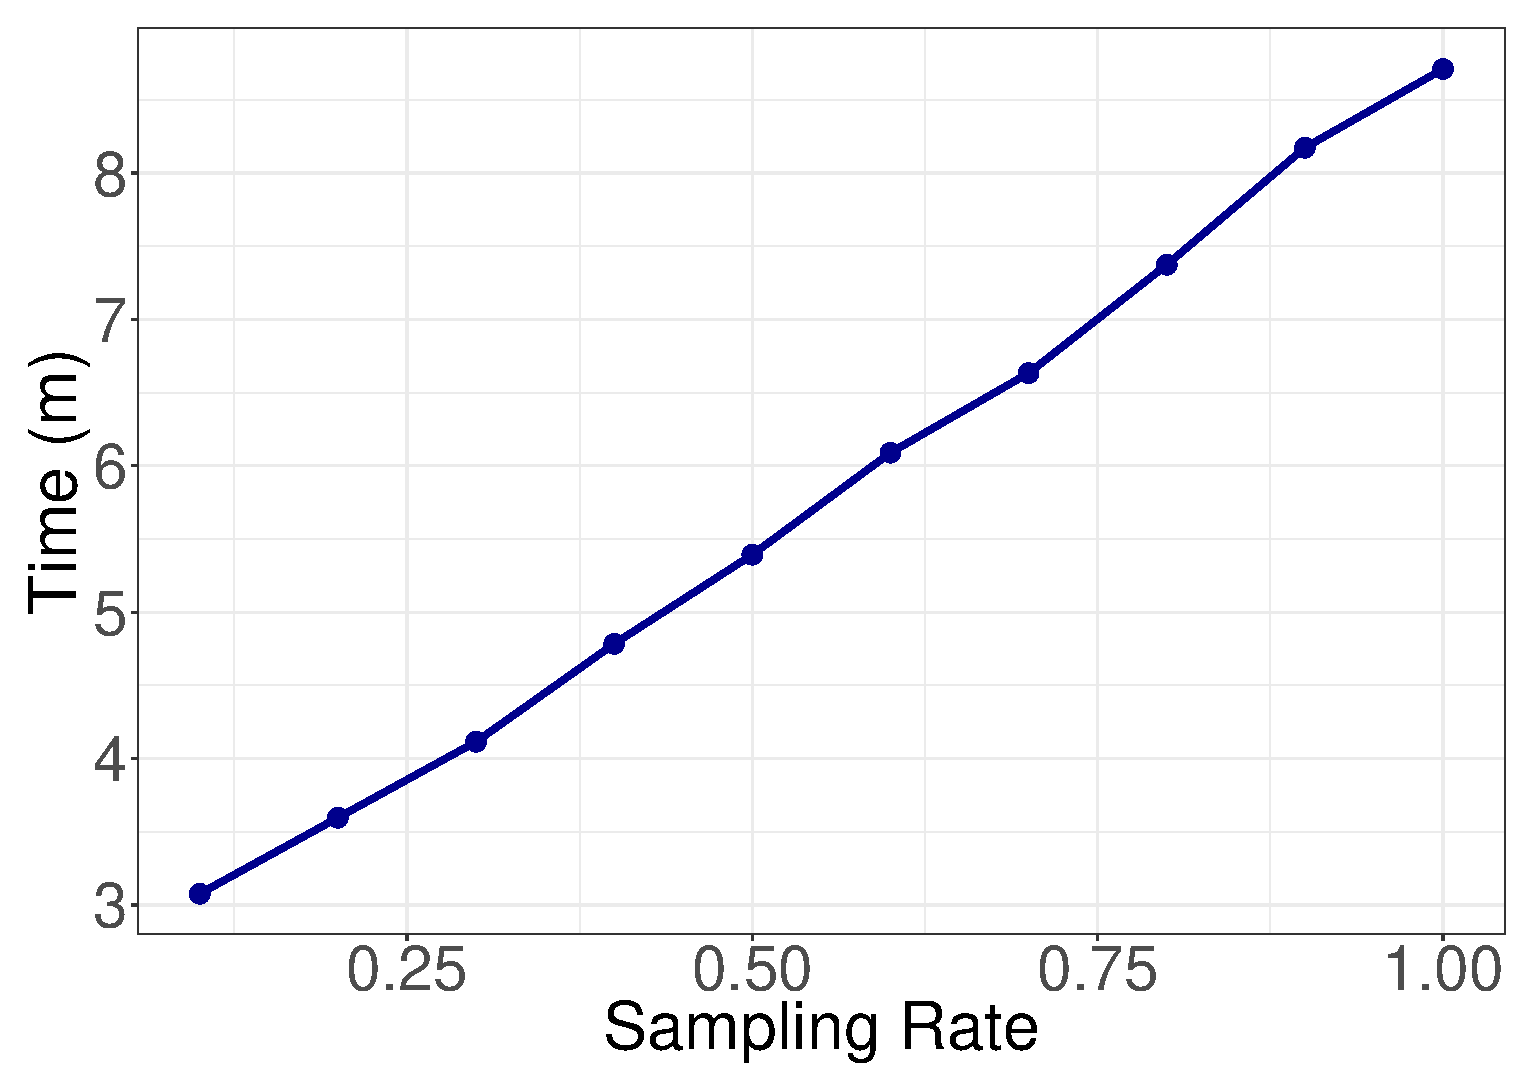
\includegraphics[width=\columnwidth]{../images/experiment-results/movie-lens-100k-sampling-time-improved.eps}
\caption{}
\label{fig:movie-lens-100k-sample-rate-time}
\end{subfigure}
\vspace{2mm}
\caption{Effect of Sampling and Scheduling Rate on Running time (Movie Lens 100K)}
\end{figure}

\todo[inline]{R1: Dynamic Scheduling is an interesting idea -- but you're not offering any scheduling algorithm here? Just the idea that you can schedule training when there's free CPU cycles? BD: Scheduling and Sampling rate have to be studied in more detail. All reviewers had concerns about these}
\todo[inline]{R3: What is exactly the scheduling?}
\textit{Dynamic scheduling:} In production environments, the load on the system typically varies throughout the lifetime of the application.
Therefore, a dynamic scheduling maximizes the performance of the system, by performing more frequent updates while there are more resources available for training. 
\todo[inline]{R1: "Moreover, since training and serving ... only update the weights when the training iteration is over". Why? Why not apply the updates to the model in-place? This allows you to serve every request with the absolute freshest model. At least for the single-machine case. BD: the updated model is the result of the training iterations, therefore, we have to wait until the iteration is over. The sentence seems clear to me. I should it run it by TR}
Moreover, since training and serving can be done in parallel, we can perform training in a background process and only update the weights when the training iteration is over. 


\subsection{Prediction Quality}
Quality achieved continuous compared with retraining method.
\begin{figure}[h]
\centering
\includegraphics[width=\columnwidth]{../images/placeholder.jpeg}
\caption{Log Loss Continuous vs Daily retraining Criteo }
\label{fig:continuous-vs-daily-criteo}
\vspace{2mm}
\end{figure}


\subsection{Serving Metrics}
\textbf{Model Freshness. }
How recent the pipeline was trained. 
The lower the value, the better quality the predictions are since they are made by a more recent model.
\begin{figure}[h]
\centering
\includegraphics[width=\columnwidth]{../images/placeholder.jpeg}
\caption{Model Freshness for deployment scenarios}
\label{fig:model-freshness-criteo}
\vspace{2mm}
\end{figure}
\textbf{Prediction Latency. }

\subsection{Training Time}
Total time spent training the pipeline for each scenario.
\begin{figure}[h]
\centering
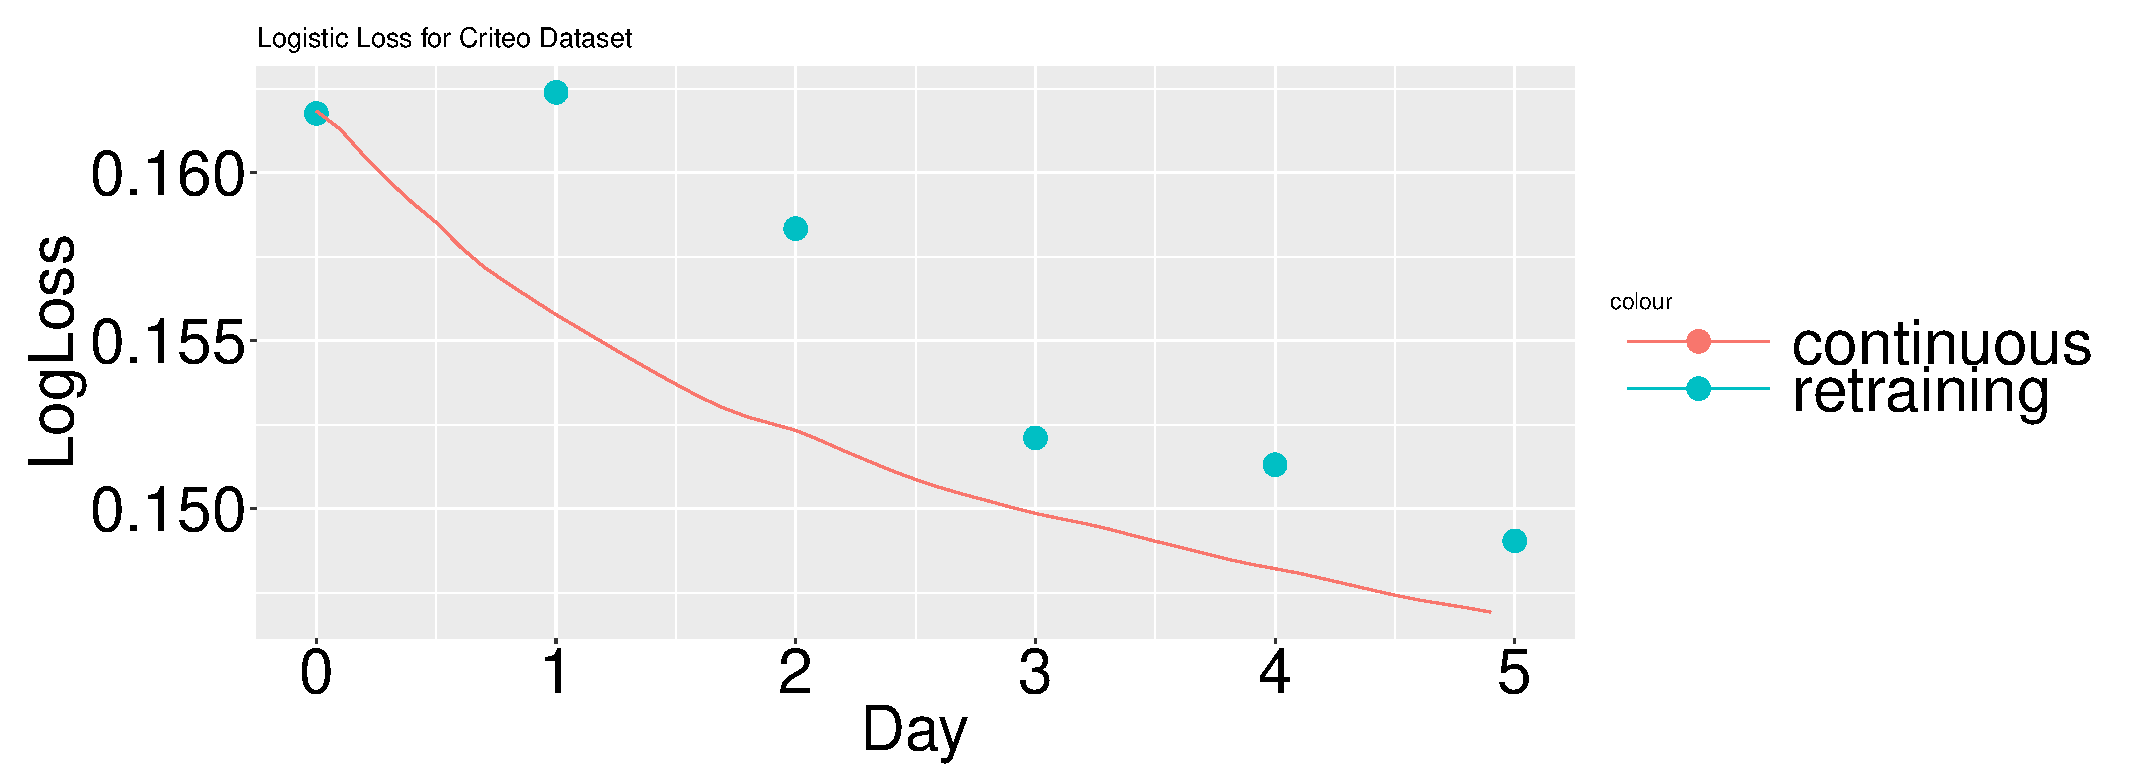
\includegraphics[width=\columnwidth]{../images/experiment-results/criteo-log-loss-continuous-vs-daily.eps}
\caption{Total training time of the pipeline for each scenario}
\label{fig:training-time-criteo}
\vspace{2mm}
\end{figure}

\subsection{Discussion} \label{subsec:discussion}
\begin{figure*}[t]
\begin{subfigure}{0.30\textwidth}
  \centering
  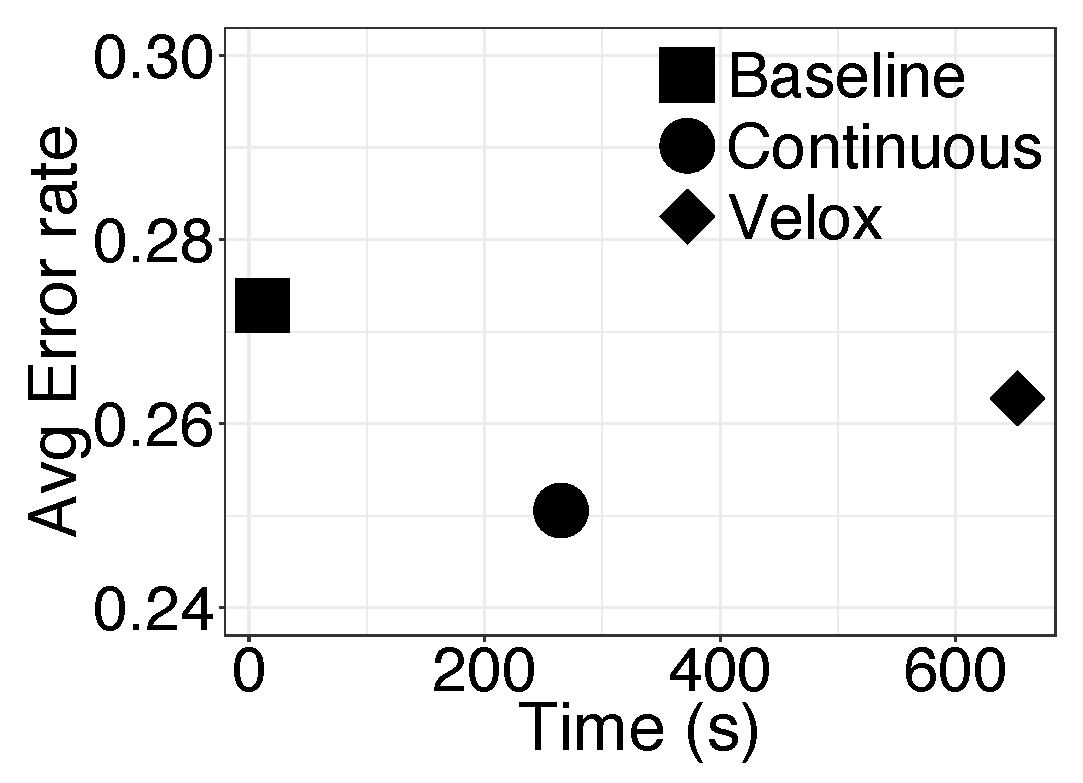
\includegraphics[width=\linewidth]{../images/experiment-results/cover-types-meta-performance.eps}
  \caption{Cover Type}
  \label{subfig:cover-type-meta}
\end{subfigure}%
  \hspace*{10mm}
\begin{subfigure}{0.30\textwidth}
 \centering
  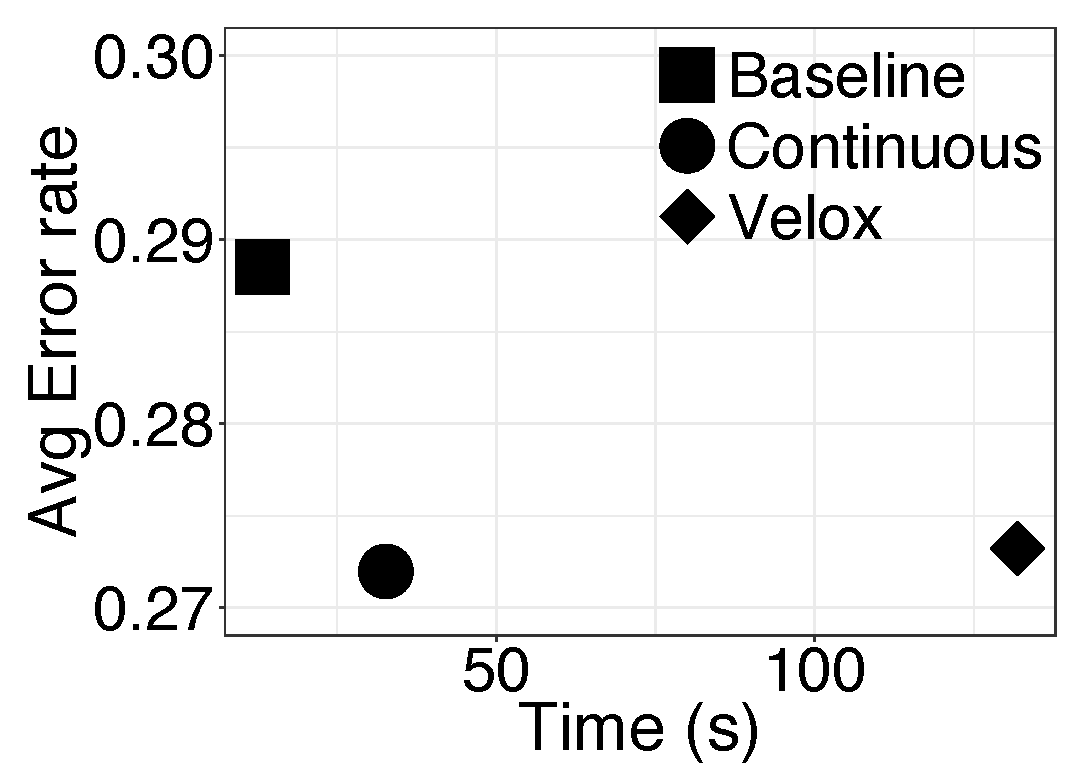
\includegraphics[width=\linewidth]{../images/experiment-results/sea-meta-performance.eps}
  \caption{SEA}
  \label{subfig:sea-meta}
\end{subfigure}%
 \hspace*{10mm}
 \begin{subfigure}{0.30\textwidth}
 \centering
  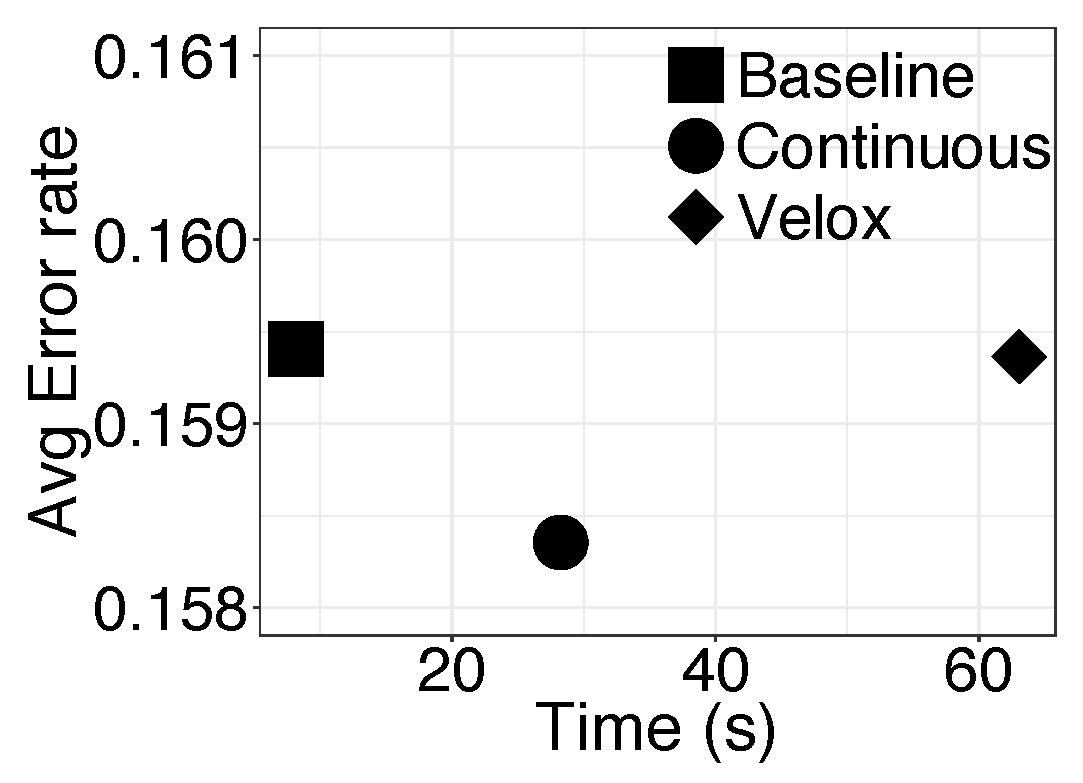
\includegraphics[width=\linewidth]{../images/experiment-results/adult-meta-performance.eps}
  \caption{Adult}
  \label{subfig:adult-meta}
\end{subfigure}%
 \vspace*{5mm}
\centering

\begin{subfigure}{.30\textwidth}
  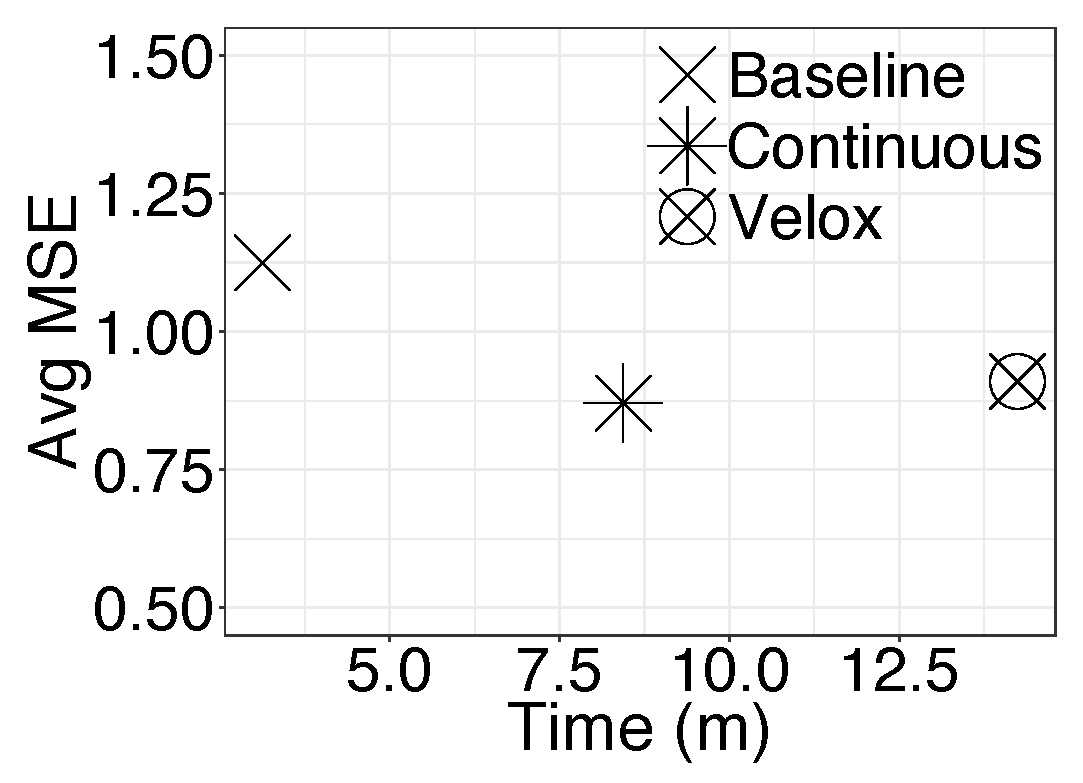
\includegraphics[width=1\linewidth, height=1\linewidth, keepaspectratio]{../images/experiment-results/movie-lens-100k-meta-performance.eps}
  \caption{Movie Lens 100K}
  \label{subfig:movie-lens-100k-meta}
\end{subfigure}%
 \hspace*{10mm}
\begin{subfigure}{0.30\textwidth}
  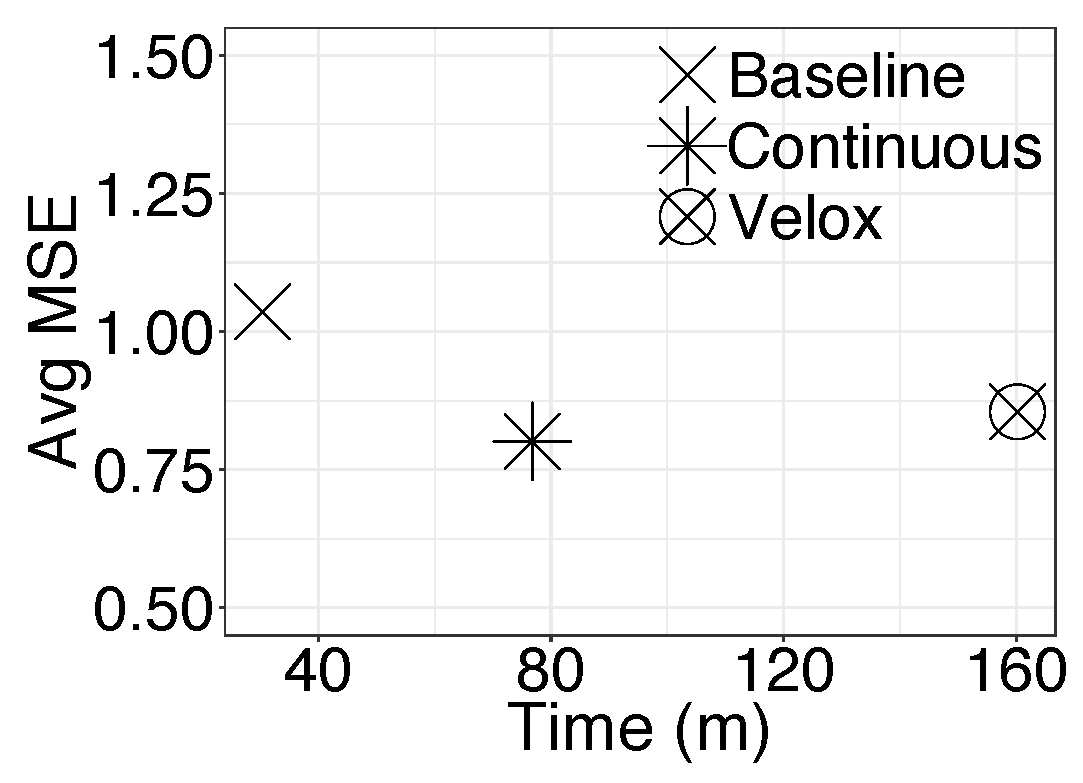
\includegraphics[width=1\linewidth, height=1\linewidth, keepaspectratio]{../images/experiment-results/movie-lens-1m-meta-performance.eps}
  \caption{Movie Lens 1M}
  \label{subfig:movie-lens-1m-meta}
\end{subfigure}


\begin{subfigure}{0.30\textwidth}
  \centering
  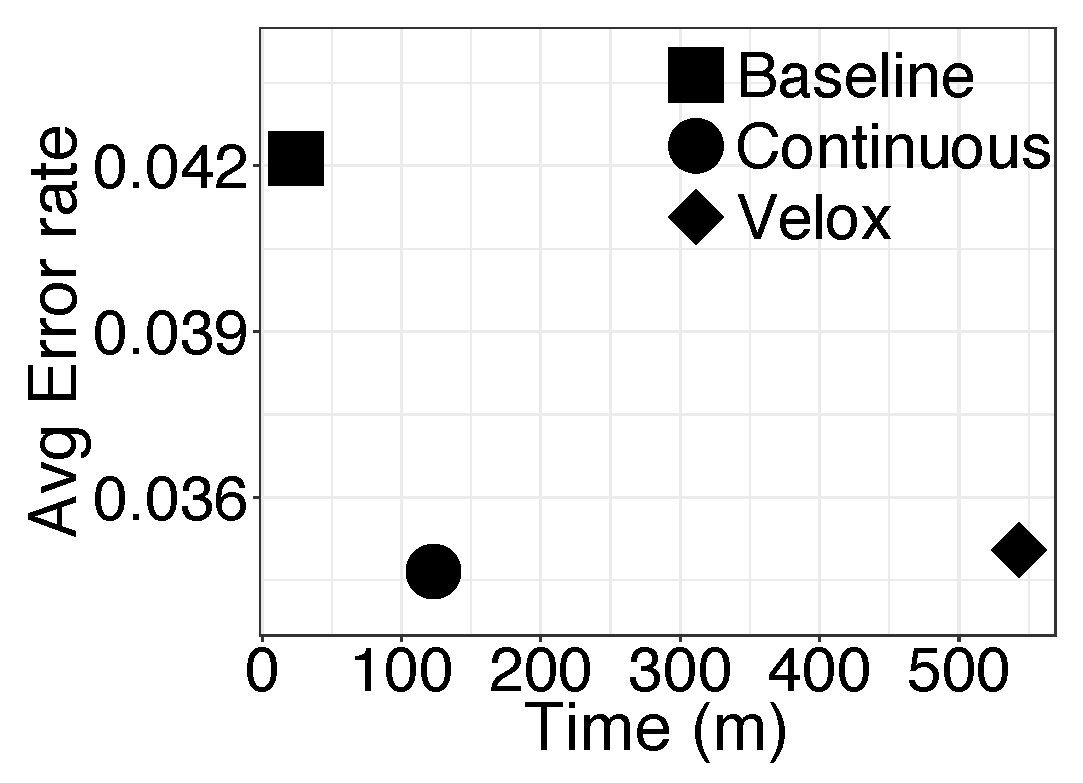
\includegraphics[width=\linewidth]{../images/experiment-results/url-reputation-meta-performance.eps}
  \caption{URL Reputation}
   \label{subfig:url-meta}
\end{subfigure}%
 \hspace*{10mm}
\begin{subfigure}{0.30\textwidth}
 \centering
  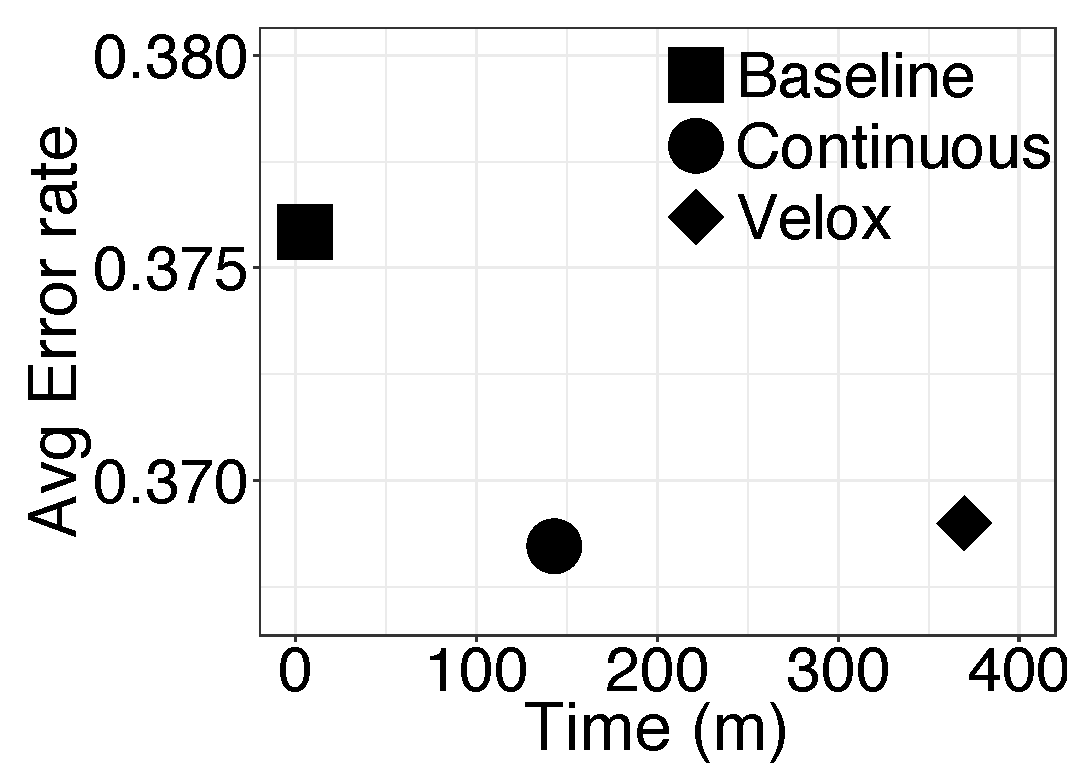
\includegraphics[width=\linewidth]{../images/experiment-results/higgs-meta-performance.eps}
  \caption{Higgs}
   \label{subfig:higgs-meta}
\end{subfigure}
 \vspace*{5mm}
\centering

\vspace{2mm}
\caption{Total Training Time vs Quality}
\label{fig:training-time-vs-quality}
\end{figure*}

Figure \ref{fig:training-time-vs-quality} shows the total training time and average error rate of each of the three different deployment methods (Baseline, Continuous, and Velox) on different datasets.
For all of the evaluated datasets, Continuous achieves the lowest average error rate (for the classification datasets) and average mean squared error (for the recommender system datasets).

The difference in average error rate (or average MSE) between Velox and Continuous is smaller for datasets that contain concept drift (Figure \ref{subfig:sea-meta}, \ref{subfig:movie-lens-100k-meta}, \ref{subfig:movie-lens-1m-meta}, and \ref{subfig:url-meta}).
Since both Velox and Continuous perform incremental and batch training of the model after it is deployed, they both manage to handle the concept drift in the data.
However, Continuous is able to adapt to the changes faster as it is continuously updating the model by executing iterations of SGD.
Since the retraining process is resource intensive, Velox cannot execute it frequently.
As a result, the underlying model in Velox cannot adapt to the changes in the distribution as quickly as Continuous.
The performance of Baseline is very poor in datasets with concept drift.
This is expected, as the underlying model in Baseline is only trained on an initial dataset.
Therefore, it is not capable of adapting to the changes in the data.

Continuous performs very well for datasets with no concept drifts (Figure \ref{subfig:cover-type-meta},  \ref{subfig:adult-meta}, and \ref{subfig:higgs-meta}) as well.
For the Cover Type and Higgs datasets, Baseline does not converge on the initial dataset, therefore it has a higher error rate than Velox and Continuous.
Velox performs better than Baseline on Higgs and Cover Type, however, retraining on these two datasets causes the underlying model to overfit to the existing data.
As a result, the performance of the model is decreased after each retraining.
This leads to an overall lower average error rate than that of Continuous.

As expected, Baseline has the lowest training time for all the datasets since it only trains the model only once on the initial datasets.
The total training time for Continuous is 2 to 5 time smaller than Velox for every datasets.
This has a big impact on prediction latency and accuracy.
In our current prototype, we do not address the problem of the trade off between prediction latency and accuracy.
In our prototype, both prediction and model updates are managed by the same node.
As a result, the prediction component is paused until the SGD iteration (or retraining in the case of Velox) is executed.
Therefore, the system always answers each prediction query using the latest version of the model, although with a much greater delay.
However, in an actual model deployment system, model training and prediction answering are typically executed on separate nodes (or threads).
Therefore, any prediction request arriving at the system is answered immediately, although not with the latest version of the model.
Since the retraining time for Velox is large, a considerable percentage of prediction requests are always answered by an older version of the model.
As a result, while the system is executing a retraining, the error rate will continue to rise until the retraining is finished.
For example in the URL Reputation dataset, the average time of each retraining is 68 minutes in Velox, whereas the average time of each iteration of SGD is 1.5 minutes.
This means that in worst case scenario, the model that is answering a prediction request in Velox is outdated by 1 hour.
Our continuous deployment method reduces this delay since it is updating the underlying model constantly using smaller batches of data.



\section{Related Work} \label{related-work}
Traditional machine learning systems focus solely on training models and leave the task of deploying and maintaining these models to the users.
It has only been recently that some systems, for example LongView \cite{akdere2011case}, Velox \cite{crankshaw2014missing}, Clipper \cite{crankshaw2016clipper} , and TensorFlow Extended \cite{baylor2017tfx}, have proposed architectures that also consider model deployment and query answering.

LongView integrates predictive machine learning models into relational databases. 
It answers predictive queries and maintains and manages the models.
LongView uses techniques such as query optimization and materialized view selection to increase the performance of the system.
However, it only works with batch data and does not provide support for real-time queries. 
As a result it does not support incremental learning.
In contrast, our system is designed to work in a dynamic environment where it answers prediction queries in real-time and incrementally updates the model when required.

Velox is an implementation of the common machine learning serving practice.
Velox supports incremental learning and can answer prediction queries in real-time.
It also eliminates the need for users to manually retrain the model offline and redeploy it again.
Velox monitors the error rate of the model using a validation set.
Once the error rate exceeds a predefined threshold, Velox initiates a complete retraining of the model using Spark. 
This deployment method, however, has three drawbacks; retraining discards updates that have been applied to the model so far, the process of retraining on full data set is resource intensive and time consuming, and new datasets introduced to the system only influence the model after the next retraining.
Our approach differs, as it exploits the underlying properties of SGD to fully integrate the training process into the system's lifeline.
This eliminates the need for completely retraining the model and replaces it with consecutive SGD-iterations.
Moreover, our system can train the model on new batch datasets as soon as they become available.

Clipper is another machine learning deployment system that focuses on producing higher quality predictions by maintaining an ensemble of models.
It constantly examines the confidence of each model.
For each prediction request, it uses the model with the highest confidence.
However, it does not incrementally train the models in production, which over time leads to models becoming outdated.
Our deployment method on the other hand, focuses on maintenance and continuous updates of the models.

TensorFlow Extended (TFX) is a platform that provides continuous training and deployment of machine learning models.
TFX automatically stores new training data, performs analysis and validation of the data, retrain new and fresh models, and finally redeploy the new models. 
However, data analysis and validation and model retraining are done periodically on batch datasets.
As a result, TFX targets use cases that typically require daily updates to the model as the overhead of performing more frequent training and data analysis is too high.
TFX provides warmstarting optimization to speed up the process of training new and fresh models.
Our continuous training method can be used as a replacement of the continuous training component of TFX.
By exploiting the properties of SGD optimization technique, our continuous training method can provide more fresh and up-to-date models (seconds to minutes instead of several hours or days) without increasing the overhead.

Weka \cite{hall2009weka}, Apache Mahout \cite{Owen:2011:MA:2132656}, and Madlib \cite{hellerstein2012madlib} are systems that provide the necessary toolkits to train machine learning models. 
All of these systems provide a range training algorithms for machine learning methods. 
However, they do not provide any management, before or after the models have been deployed. 
Our proposed system focuses on models trainable using stochastic gradient descent and as a result is able to provide model management both during training and deployment time.

MLBase \cite{kraska2013mlbase} and TuPaq \cite{sparks2015tupaq} are model management systems.
They provide a range of training algorithms to create machine learning models and mechanism for model search as well as model management.
They focus on training high quality models by performing automatic feature engineering and hyper-parameter search.
However, they only work with batch datasets.
Once models are trained, they have to be deployed and used for serving manually by the users.
Our system, on the contrary, is designed for deployment and maintenance of already trained models.

\section{Conclusions} \label{conclusion}
We propose a deployment platform for continuously updating machine learning pipelines and models.
After a machine learning pipeline is designed and initially trained on a dataset, our platform deploys the pipeline and makes it available for answering prediction queries.

To guarantee a model with an acceptable error rate, existing deployment platforms periodically train the deployed model. 
However, periodical training is a time-consuming and resource-intensive process.
As a result of the lengthy training process, the platform cannot produce fresh models.
This results in model-staleness and a drop in the quality of the deployed model.

We propose a training approach, called proactive training, that utilizes samples of historical data to train the deployed pipeline.
Proactive training replaces the periodical retraining, thus guaranteeing a high-quality model with the lengthy retraining process.
We also propose online statistics computation and materialization of the preprocessed features.
We propose a modular design that enables our deployment platform to be integrated with different scalable data processing platforms.

We implement a prototype using Apache Spark to evaluate the performance of our deployment platform on different datasets.
In our experiments, we develop two pipelines with different machine learning models to process two different datasets.
We discuss how to tune the deployment platform based on the available historical data.
Our experiments show that our continuous deployment reduces the total training cost by a factor $5$ and $13$ for the Taxi and URL datasets, respectively.
Moreover, continuous deployment improves the overall quality of the deployed model when compared with the periodical deployment approach.

In the future work, we will integrate more complex machine learning pipelines (e.g., neural networks) into our deployment platform and investigate the effect of concept drift and anomaly on our deployment platform.



\bibliographystyle{plain}
{\fontsize{8}{4}\selectfont \bibliography{references}}
\end{document}